\documentclass[11pt]{report}

\newcommand{\coursetitle}{Fundamentals of Deep Learning}
% ============================================================
%  Shared preamble for all course notes
%  Loaded from each course's main.tex via % ============================================================
%  Shared preamble for all course notes
%  Loaded from each course's main.tex via % ============================================================
%  Shared preamble for all course notes
%  Loaded from each course's main.tex via \input{../common/preamble}
% ============================================================

% ---------- Page layout & fonts ----------
\usepackage[utf8]{inputenc}
\usepackage[T1]{fontenc}
\usepackage{lmodern}
\usepackage{microtype}
\usepackage[a4paper, margin=2.5cm]{geometry}
\usepackage{parskip}               % space between paragraphs, no indent
\usepackage{fancyhdr}

% ---------- Math ----------
\usepackage{amsmath, amssymb, amsthm}
\usepackage{mathtools}
\usepackage{bm}

% ---------- Figures, tables, plots ----------
\usepackage{graphicx}
\usepackage{float}
\usepackage{caption}
\usepackage{subcaption}
\usepackage{booktabs}
\usepackage{tikz}
\usetikzlibrary{arrows.meta, positioning, shapes, calc, fit}
\usepackage{pgfplots}
\pgfplotsset{compat=1.17}
\graphicspath{{figures/}}

% ---------- Lists, code, colored boxes ----------
\usepackage{enumitem}
\usepackage{xcolor}
\usepackage{listings}
\usepackage[most]{tcolorbox}

% ---------- References ----------
\usepackage[numbers]{natbib}
\usepackage[colorlinks=true, linkcolor=blue!60!black,
            citecolor=green!50!black, urlcolor=blue!70!black]{hyperref}
\usepackage[capitalise, noabbrev]{cleveref}   % must come after hyperref

% ---------- Header / footer ----------
\pagestyle{fancy}
\fancyhf{}
\fancyhead[L]{\nouppercase{\leftmark}}
\fancyhead[R]{\coursetitle}
\fancyfoot[C]{\thepage}
\setlength{\headheight}{14.5pt}

% ---------- Theorem-like environments ----------
\theoremstyle{definition}
\newtheorem{definition}{Definition}[chapter]
\newtheorem{example}{Example}[chapter]
\newtheorem{exercise}{Exercise}[chapter]

\theoremstyle{plain}
\newtheorem{theorem}{Theorem}[chapter]
\newtheorem{lemma}[theorem]{Lemma}
\newtheorem{proposition}[theorem]{Proposition}
\newtheorem{corollary}[theorem]{Corollary}

\theoremstyle{remark}
\newtheorem*{remark}{Remark}
\newtheorem*{note}{Note}

% ---------- Highlight boxes ----------
% \begin{keyidea} ... \end{keyidea}   -- main takeaway of a lecture
% \begin{intuition} ... \end{intuition}
\newtcolorbox{keyidea}[1][Key Idea]{
  colback=blue!4, colframe=blue!50!black, fonttitle=\bfseries,
  title=#1, breakable}
\newtcolorbox{intuition}[1][Intuition]{
  colback=green!4, colframe=green!40!black, fonttitle=\bfseries,
  title=#1, breakable}
\newtcolorbox{warning}[1][Caution]{
  colback=red!4, colframe=red!50!black, fonttitle=\bfseries,
  title=#1, breakable}

% ---------- Code listings (Python by default) ----------
\lstdefinestyle{notes}{
  language=Python,
  basicstyle=\ttfamily\small,
  keywordstyle=\color{blue!70!black}\bfseries,
  commentstyle=\color{green!45!black}\itshape,
  stringstyle=\color{red!60!black},
  numbers=left, numberstyle=\tiny\color{gray},
  frame=single, rulecolor=\color{gray!40},
  backgroundcolor=\color{gray!5},
  breaklines=true, showstringspaces=false, tabsize=4,
  captionpos=b
}
\lstset{style=notes}

% ---------- Shared math notation ----------
\input{../common/macros}

% ============================================================

% ---------- Page layout & fonts ----------
\usepackage[utf8]{inputenc}
\usepackage[T1]{fontenc}
\usepackage{lmodern}
\usepackage{microtype}
\usepackage[a4paper, margin=2.5cm]{geometry}
\usepackage{parskip}               % space between paragraphs, no indent
\usepackage{fancyhdr}

% ---------- Math ----------
\usepackage{amsmath, amssymb, amsthm}
\usepackage{mathtools}
\usepackage{bm}

% ---------- Figures, tables, plots ----------
\usepackage{graphicx}
\usepackage{float}
\usepackage{caption}
\usepackage{subcaption}
\usepackage{booktabs}
\usepackage{tikz}
\usetikzlibrary{arrows.meta, positioning, shapes, calc, fit}
\usepackage{pgfplots}
\pgfplotsset{compat=1.17}
\graphicspath{{figures/}}

% ---------- Lists, code, colored boxes ----------
\usepackage{enumitem}
\usepackage{xcolor}
\usepackage{listings}
\usepackage[most]{tcolorbox}

% ---------- References ----------
\usepackage[numbers]{natbib}
\usepackage[colorlinks=true, linkcolor=blue!60!black,
            citecolor=green!50!black, urlcolor=blue!70!black]{hyperref}
\usepackage[capitalise, noabbrev]{cleveref}   % must come after hyperref

% ---------- Header / footer ----------
\pagestyle{fancy}
\fancyhf{}
\fancyhead[L]{\nouppercase{\leftmark}}
\fancyhead[R]{\coursetitle}
\fancyfoot[C]{\thepage}
\setlength{\headheight}{14.5pt}

% ---------- Theorem-like environments ----------
\theoremstyle{definition}
\newtheorem{definition}{Definition}[chapter]
\newtheorem{example}{Example}[chapter]
\newtheorem{exercise}{Exercise}[chapter]

\theoremstyle{plain}
\newtheorem{theorem}{Theorem}[chapter]
\newtheorem{lemma}[theorem]{Lemma}
\newtheorem{proposition}[theorem]{Proposition}
\newtheorem{corollary}[theorem]{Corollary}

\theoremstyle{remark}
\newtheorem*{remark}{Remark}
\newtheorem*{note}{Note}

% ---------- Highlight boxes ----------
% \begin{keyidea} ... \end{keyidea}   -- main takeaway of a lecture
% \begin{intuition} ... \end{intuition}
\newtcolorbox{keyidea}[1][Key Idea]{
  colback=blue!4, colframe=blue!50!black, fonttitle=\bfseries,
  title=#1, breakable}
\newtcolorbox{intuition}[1][Intuition]{
  colback=green!4, colframe=green!40!black, fonttitle=\bfseries,
  title=#1, breakable}
\newtcolorbox{warning}[1][Caution]{
  colback=red!4, colframe=red!50!black, fonttitle=\bfseries,
  title=#1, breakable}

% ---------- Code listings (Python by default) ----------
\lstdefinestyle{notes}{
  language=Python,
  basicstyle=\ttfamily\small,
  keywordstyle=\color{blue!70!black}\bfseries,
  commentstyle=\color{green!45!black}\itshape,
  stringstyle=\color{red!60!black},
  numbers=left, numberstyle=\tiny\color{gray},
  frame=single, rulecolor=\color{gray!40},
  backgroundcolor=\color{gray!5},
  breaklines=true, showstringspaces=false, tabsize=4,
  captionpos=b
}
\lstset{style=notes}

% ---------- Shared math notation ----------
% ============================================================
%  Shared math notation for ML / DL notes
% ============================================================

% ---------- Number sets ----------
\newcommand{\R}{\mathbb{R}}
\newcommand{\N}{\mathbb{N}}
\newcommand{\Z}{\mathbb{Z}}

% ---------- Probability ----------
\newcommand{\E}{\mathbb{E}}
\newcommand{\Prob}{\mathbb{P}}
\DeclareMathOperator{\Var}{Var}
\DeclareMathOperator{\Cov}{Cov}
\newcommand{\KL}[2]{D_{\mathrm{KL}}\!\left(#1 \,\|\, #2\right)}
\newcommand{\Normal}{\mathcal{N}}
\newcommand{\iid}{\overset{\text{i.i.d.}}{\sim}}

% ---------- Linear algebra ----------
\renewcommand{\vec}[1]{\bm{#1}}          % vectors: \vec{x}
\newcommand{\mat}[1]{\bm{#1}}            % matrices: \mat{W}
\newcommand{\T}{^{\top}}                 % transpose: \vec{x}\T
\DeclareMathOperator{\tr}{tr}
\DeclareMathOperator{\rank}{rank}
\DeclareMathOperator{\diag}{diag}
\DeclarePairedDelimiter{\norm}{\lVert}{\rVert}
\DeclarePairedDelimiter{\abs}{\lvert}{\rvert}
\DeclarePairedDelimiter{\inner}{\langle}{\rangle}

% ---------- Optimization / calculus ----------
\DeclareMathOperator*{\argmin}{arg\,min}
\DeclareMathOperator*{\argmax}{arg\,max}
\newcommand{\grad}{\nabla}
\newcommand{\pd}[2]{\frac{\partial #1}{\partial #2}}

% ---------- ML-specific ----------
\newcommand{\dataset}{\mathcal{D}}
\newcommand{\loss}{\mathcal{L}}
\newcommand{\hypo}{\mathcal{H}}
\newcommand{\params}{\bm{\theta}}
\newcommand{\X}{\mathcal{X}}
\newcommand{\Y}{\mathcal{Y}}
\newcommand{\indicator}[1]{\mathbb{1}\!\left[#1\right]}
\DeclareMathOperator{\sigmoid}{\sigma}
\DeclareMathOperator{\softmax}{softmax}
\DeclareMathOperator{\ReLU}{ReLU}
\DeclareMathOperator{\sign}{sign}


% ============================================================

% ---------- Page layout & fonts ----------
\usepackage[utf8]{inputenc}
\usepackage[T1]{fontenc}
\usepackage{lmodern}
\usepackage{microtype}
\usepackage[a4paper, margin=2.5cm]{geometry}
\usepackage{parskip}               % space between paragraphs, no indent
\usepackage{fancyhdr}

% ---------- Math ----------
\usepackage{amsmath, amssymb, amsthm}
\usepackage{mathtools}
\usepackage{bm}

% ---------- Figures, tables, plots ----------
\usepackage{graphicx}
\usepackage{float}
\usepackage{caption}
\usepackage{subcaption}
\usepackage{booktabs}
\usepackage{tikz}
\usetikzlibrary{arrows.meta, positioning, shapes, calc, fit}
\usepackage{pgfplots}
\pgfplotsset{compat=1.17}
\graphicspath{{figures/}}

% ---------- Lists, code, colored boxes ----------
\usepackage{enumitem}
\usepackage{xcolor}
\usepackage{listings}
\usepackage[most]{tcolorbox}

% ---------- References ----------
\usepackage[numbers]{natbib}
\usepackage[colorlinks=true, linkcolor=blue!60!black,
            citecolor=green!50!black, urlcolor=blue!70!black]{hyperref}
\usepackage[capitalise, noabbrev]{cleveref}   % must come after hyperref

% ---------- Header / footer ----------
\pagestyle{fancy}
\fancyhf{}
\fancyhead[L]{\nouppercase{\leftmark}}
\fancyhead[R]{\coursetitle}
\fancyfoot[C]{\thepage}
\setlength{\headheight}{14.5pt}

% ---------- Theorem-like environments ----------
\theoremstyle{definition}
\newtheorem{definition}{Definition}[chapter]
\newtheorem{example}{Example}[chapter]
\newtheorem{exercise}{Exercise}[chapter]

\theoremstyle{plain}
\newtheorem{theorem}{Theorem}[chapter]
\newtheorem{lemma}[theorem]{Lemma}
\newtheorem{proposition}[theorem]{Proposition}
\newtheorem{corollary}[theorem]{Corollary}

\theoremstyle{remark}
\newtheorem*{remark}{Remark}
\newtheorem*{note}{Note}

% ---------- Highlight boxes ----------
% \begin{keyidea} ... \end{keyidea}   -- main takeaway of a lecture
% \begin{intuition} ... \end{intuition}
\newtcolorbox{keyidea}[1][Key Idea]{
  colback=blue!4, colframe=blue!50!black, fonttitle=\bfseries,
  title=#1, breakable}
\newtcolorbox{intuition}[1][Intuition]{
  colback=green!4, colframe=green!40!black, fonttitle=\bfseries,
  title=#1, breakable}
\newtcolorbox{warning}[1][Caution]{
  colback=red!4, colframe=red!50!black, fonttitle=\bfseries,
  title=#1, breakable}

% ---------- Code listings (Python by default) ----------
\lstdefinestyle{notes}{
  language=Python,
  basicstyle=\ttfamily\small,
  keywordstyle=\color{blue!70!black}\bfseries,
  commentstyle=\color{green!45!black}\itshape,
  stringstyle=\color{red!60!black},
  numbers=left, numberstyle=\tiny\color{gray},
  frame=single, rulecolor=\color{gray!40},
  backgroundcolor=\color{gray!5},
  breaklines=true, showstringspaces=false, tabsize=4,
  captionpos=b
}
\lstset{style=notes}

% ---------- Shared math notation ----------
% ============================================================
%  Shared math notation for ML / DL notes
% ============================================================

% ---------- Number sets ----------
\newcommand{\R}{\mathbb{R}}
\newcommand{\N}{\mathbb{N}}
\newcommand{\Z}{\mathbb{Z}}

% ---------- Probability ----------
\newcommand{\E}{\mathbb{E}}
\newcommand{\Prob}{\mathbb{P}}
\DeclareMathOperator{\Var}{Var}
\DeclareMathOperator{\Cov}{Cov}
\newcommand{\KL}[2]{D_{\mathrm{KL}}\!\left(#1 \,\|\, #2\right)}
\newcommand{\Normal}{\mathcal{N}}
\newcommand{\iid}{\overset{\text{i.i.d.}}{\sim}}

% ---------- Linear algebra ----------
\renewcommand{\vec}[1]{\bm{#1}}          % vectors: \vec{x}
\newcommand{\mat}[1]{\bm{#1}}            % matrices: \mat{W}
\newcommand{\T}{^{\top}}                 % transpose: \vec{x}\T
\DeclareMathOperator{\tr}{tr}
\DeclareMathOperator{\rank}{rank}
\DeclareMathOperator{\diag}{diag}
\DeclarePairedDelimiter{\norm}{\lVert}{\rVert}
\DeclarePairedDelimiter{\abs}{\lvert}{\rvert}
\DeclarePairedDelimiter{\inner}{\langle}{\rangle}

% ---------- Optimization / calculus ----------
\DeclareMathOperator*{\argmin}{arg\,min}
\DeclareMathOperator*{\argmax}{arg\,max}
\newcommand{\grad}{\nabla}
\newcommand{\pd}[2]{\frac{\partial #1}{\partial #2}}

% ---------- ML-specific ----------
\newcommand{\dataset}{\mathcal{D}}
\newcommand{\loss}{\mathcal{L}}
\newcommand{\hypo}{\mathcal{H}}
\newcommand{\params}{\bm{\theta}}
\newcommand{\X}{\mathcal{X}}
\newcommand{\Y}{\mathcal{Y}}
\newcommand{\indicator}[1]{\mathbb{1}\!\left[#1\right]}
\DeclareMathOperator{\sigmoid}{\sigma}
\DeclareMathOperator{\softmax}{softmax}
\DeclareMathOperator{\ReLU}{ReLU}
\DeclareMathOperator{\sign}{sign}



% ------------------------------------------------------------
% Compile only some chapters while working on them (faster).
% Uncomment and list the chapters you want; the rest are skipped
% but numbering and cross-references are kept.
% ------------------------------------------------------------
% \includeonly{chapters/01_logreg_to_mlp}

\title{\textbf{\coursetitle} \\ \large Lecture Notes}
\author{Muxammadrizo Maribjonov}
\date{\today}

\begin{document}

\maketitle
\tableofcontents

% ---------------- Chapters (one file each) ----------------
% ============================================================
%  Chapter 1: From Logistic Regression to MLPs
% ============================================================
\chapter{From Logistic Regression to MLPs}
\label{ch:logreg_to_mlp}

% Section 1.1: self-contained derivation, figures and NumPy companion.
\section{Recap of Logistic Regression}
\label{sec:logreg_to_mlp:recap_of_logistic_regression}

\begin{keyidea}[The question behind every formula]
A classifier must decide what to do, but first it can estimate what might be true.
Logistic regression separates these two tasks: a model assigns a probability to a
binary outcome, and a decision rule turns that probability into an action.
The sigmoid specifies the probability model; cross-entropy measures how much
probability that model assigned to the outcome actually observed.
\end{keyidea}

\subsection{The problem: a decision is not a probability}
Imagine a robot about to grasp a cup. From its camera and estimated gripper pose,
it measures a centering error and an angular misalignment. The outcome is
$Y=1$ for a successful grasp and $Y=0$ for a failure. We would like to answer
both ``How likely is success?'' and ``Should the robot attempt this grasp?''
These are different questions. A success probability of $0.7$ might justify a
cheap retryable grasp but not a grasp whose failure breaks an expensive object.

Why not just fit a line to the labels? A real-valued affine prediction can be
negative or greater than one. Why not immediately threshold that line? A hard
threshold throws away the distinction between a barely positive score and a
strongly positive score. It also gives a piecewise constant classification error,
which offers little useful gradient information. We therefore seek a smooth
conditional probability model before choosing a decision rule.

This section develops the connected chain
\[
\text{features}\longrightarrow\text{score}\longrightarrow\text{probability}
\longrightarrow\text{likelihood}\longrightarrow\text{loss}
\longrightarrow\text{learning and decisions}.
\]
We first understand a fixed model. Only later do we vary its parameters to train
it. The examples and plots here are constructed teaching examples, not empirical
claims about a deployed robot.

\subsection{Notation and the assumptions we are making}
Let $x=(x_1,\ldots,x_d)^\top\in\mathbb R^d$ denote the measured features and let
$Y\in\{0,1\}$ be a random outcome. Define the augmented input and parameter vector
\[
\tilde x=\begin{bmatrix}1\\x\end{bmatrix}\in\mathbb R^{d+1},\qquad
w=\begin{bmatrix}b\\a\end{bmatrix},\qquad
z=w^\top\tilde x=b+a^\top x.
\]
The slides call the bias $w_0$ and use $x_0=1$; thus their $w^\top x$ is our
$w^\top\tilde x$. We keep the tilde to distinguish the actual feature space from
the augmented space. The scalar $z$ is the \emph{score} or \emph{logit}.

\begin{center}
\begin{tabular}{ll}
\toprule
Symbol & Meaning \\
\midrule
$Y$ & Random binary label before observing the outcome \\
$y$ & Observed label, exactly zero or one \\
$q(x)$ & True conditional probability $\Pr(Y=1\mid X=x)$ \\
$p_w(x)$ & Model probability, also written $h_w(x)$ \\
$\hat y$ & In the slides, the probability $h_w(x)$ \\
$\hat c$ & Hard class prediction, zero or one \\
$\ell(p,y)$ & Loss on one observation \\
$J(w)$ & Mean loss over the training data \\
\bottomrule
\end{tabular}
\end{center}

\paragraph{Definitions, assumptions, consequences.}
That a binary conditional distribution is Bernoulli is a consequence of its two
possible outcomes: it is completely specified by one probability. That its
\emph{log-odds is affine in the chosen features} will be our modeling assumption.
That independent observations give a product likelihood is an additional
sampling assumption. Cross-entropy then follows from maximum likelihood; its
convexity follows from calculus. These statements play different logical roles.

Conditioning matters. We model $Y\mid X=x$, not one identical Bernoulli law for
all inputs. At different inputs the success probabilities can differ. Treating
$Y$ probabilistically does not assert that the world is fundamentally random.
Unmeasured friction, occlusion, noisy sensors, or missing features can make an
outcome unpredictable from the information we have.

\subsection{Inventing the sigmoid through odds and evidence}
A useful probability must stay in $[0,1]$, while a linear score can take any real
value. Many maps could enforce this range. Why use this particular one?

For $0<p<1$, define the \emph{odds} as $p/(1-p)$. If $p=0.8$, the odds are $4$:
success has four times the probability of failure. Odds live in $(0,\infty)$;
logarithms turn this into the whole real line. The \emph{log-odds} is
\[
\operatorname{logit}(p)=\log\frac{p}{1-p}.
\]
We now \emph{assume} that evidence measured in log-odds is additive:
\begin{equation}
\log\frac{p_w(x)}{1-p_w(x)}=b+\sum_{j=1}^d a_jx_j=z.
\label{eq:lr11-logodds}
\end{equation}
Solving, rather than memorizing, gives
\[
\frac{p}{1-p}=e^z
\quad\Longrightarrow\quad p=e^z(1-p)
\quad\Longrightarrow\quad p(1+e^z)=e^z
\quad\Longrightarrow\quad
\boxed{p_w(x)=\sigma(z)=\frac{1}{1+e^{-z}}.}
\]
This is an equivalence: affine log-odds and a sigmoid of an affine score describe
exactly the same model. Binary labels alone do not force this choice; a probit
link, for example, would define a different model.

Equation~\eqref{eq:lr11-logodds} also explains the parameters. Increasing $x_j$ by
one unit with other features held fixed multiplies the odds by $e^{a_j}$.
It does \emph{not} add $a_j$ to the probability. The bias is the log-odds at
$x=0$, so $p_w(0)=\sigma(b)$. This interpretation depends on units and on whether
zero is meaningful for the features.

\paragraph{Why additive log-odds is a reasonable idea.}
Bayes' rule gives, wherever the densities are positive,
\[
\log\frac{\Pr(Y=1\mid x)}{\Pr(Y=0\mid x)}
=\log\frac{\Pr(Y=1)}{\Pr(Y=0)}
 +\log\frac{p(x\mid Y=1)}{p(x\mid Y=0)}.
\]
Under conditional independence of features, the last term becomes a sum of
featurewise log-likelihood ratios. This motivates adding evidence. Logistic
regression itself does \emph{not} require conditional feature independence; it
models the final conditional log-odds directly. This is a conceptual motivation,
not a claim about the historical invention of the method.

\paragraph{A nontrivial case where the affine assumption is exact.}
Suppose $X\mid Y=k\sim\mathcal N(\mu_k,\Sigma)$, with the same positive-definite
covariance for both classes and priors $\pi_k>0$. The normalizing constants cancel
in the density ratio, leaving
\begin{align*}
\log\frac{q(x)}{1-q(x)}
&=\log\frac{\pi_1}{\pi_0}
-\frac12(x-\mu_1)^\top\Sigma^{-1}(x-\mu_1)
+\frac12(x-\mu_0)^\top\Sigma^{-1}(x-\mu_0)\\
&=(\mu_1-\mu_0)^\top\Sigma^{-1}x
-\frac12\bigl(\mu_1^\top\Sigma^{-1}\mu_1
             -\mu_0^\top\Sigma^{-1}\mu_0\bigr)
+\log\frac{\pi_1}{\pi_0}.
\end{align*}
The quadratic terms in $x$ cancel. Thus a Gaussian generative assumption can
produce precisely a logistic conditional model. Unequal covariances generally
leave quadratic terms. Logistic regression need not fit either Gaussian density
to learn an affine log-odds model.

\subsection{Geometry: why the boundary is a line}
For equal costs of the two mistakes, predict class one when $p_w(x)\geq 1/2$.
To understand its geometry, differentiate:
\[
\sigma'(z)=\frac{e^{-z}}{(1+e^{-z})^2}
=\sigma(z)\bigl(1-\sigma(z)\bigr)>0
\quad\text{for finite }z.
\]
The sigmoid is strictly increasing and $\sigma(0)=1/2$. Therefore
\begin{equation}
\hat c=\mathbf 1\{p_w(x)\geq 1/2\}
=\mathbf 1\{b+a^\top x\geq0\}.
\label{eq:lr11-boundary}
\end{equation}
Its decision boundary is $b+a^\top x=0$. In two dimensions this is a line; in
three, a plane; in $d$ dimensions, a hyperplane, provided $a\ne0$.
Strictly, $b+a^\top x$ is \emph{affine} in $x$ and linear in $\tilde x$.
The informal phrase ``linear classifier'' includes an affine bias.

For the slide's $w=(-3,1,1)^\top$, we obtain
\[
z=-3+x_1+x_2,\qquad x_2=3-x_1.
\]
At $(1,1)$ the score is $-1$ and $p\approx0.269$; at $(1,2)$ it is $0$ and
$p=0.5$; at $(2,2)$ it is $1$ and $p\approx0.731$; at $(4,4)$ it is $5$ and
$p\approx0.9933$. We use class one for ties by convention. Another tie convention
changes only points exactly on the boundary.

\paragraph{Direction, distance, and confidence.}
Moving by a displacement $v$ changes the score by $a^\top v$. If $a^\top v=0$,
we remain on a constant-score hyperplane. Thus $a$ is normal to the boundary.
For $a\ne0$ the signed perpendicular distance from $x$ to the boundary is
\[
\delta(x)=\frac{b+a^\top x}{\|a\|_2},\qquad
p_w(x)=\sigma\bigl(\|a\|_2\delta(x)\bigr).
\]
The score is a \emph{scaled} distance, not a distance in physical units. Scaling
all weights by $c>0$ preserves the boundary but changes the probabilities to
$\sigma(cz)$. As $c$ grows, predictions away from the boundary approach zero or
one. The same classification accuracy can hide very different probability
quality. If $c<0$, the boundary stays but class assignments reverse.

\begin{figure}[htbp]
\centering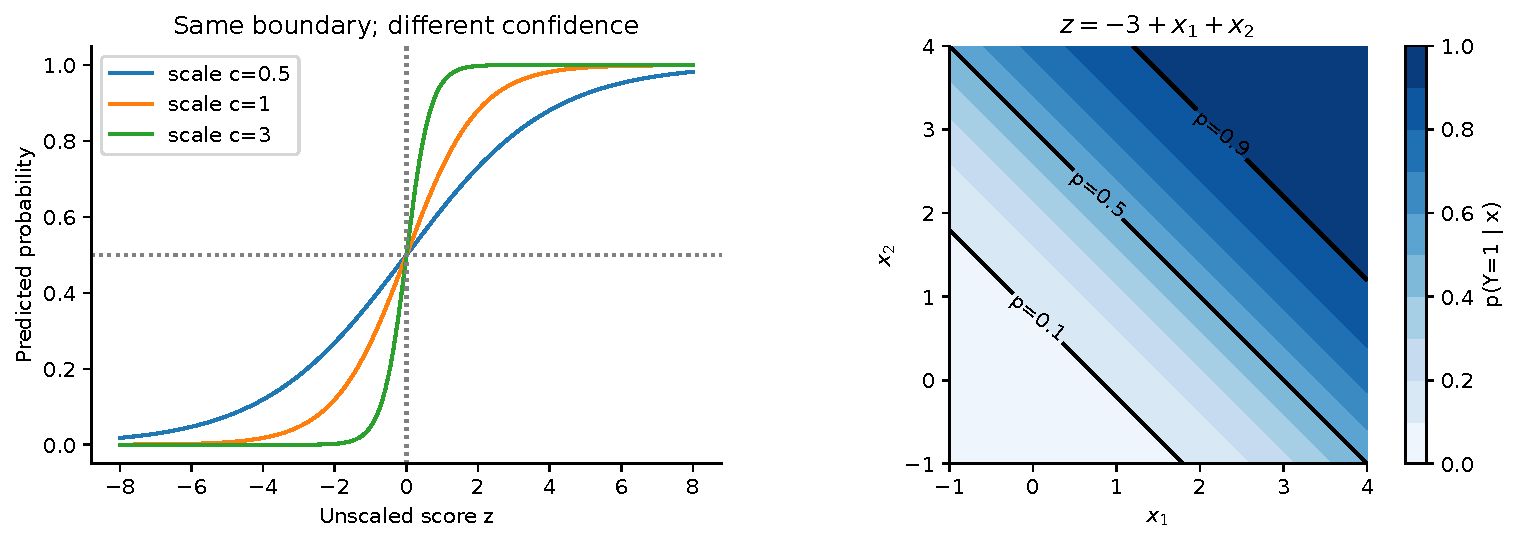
\includegraphics[width=\linewidth]{logreg_1_1/geometry.pdf}
\caption{Left: rescaling a logit changes confidence without moving the zero
threshold. Right: parallel probability contours around the boundary
$x_1+x_2=3$. The sigmoid bends the probability response, not this boundary.}
\label{fig:lr11-geometry}
\end{figure}

\paragraph{Edge cases.}
If $a=0$ and $b\ne0$, the prediction is constant and there is no boundary.
If $a=0$ and $b=0$, every point has probability $1/2$. The normalized-distance
formula cannot be used in either case.

\subsection{What does ``maximally uncertain'' actually mean?}
For a fixed model $w$, $p_w(x)$ is a deterministic number at a fixed input.
It specifies a distribution over $Y$, not a random choice of weights. The model's
Bernoulli variance is
\[
\operatorname{Var}(Y\mid x;w)=p(1-p)=\frac14-(p-\tfrac12)^2,
\]
which is largest at $p=1/2$. Its predictive entropy, in nats, is
\[
H(p)=-p\log p-(1-p)\log(1-p).
\]
Differentiation gives
\[
H'(p)=\log\frac{1-p}{p},\qquad
H''(p)=-\frac1p-\frac1{1-p}<0.
\]
So entropy has a unique maximum $H(1/2)=\log2$. This is the precise sense in which
the model is maximally uncertain at its $0.5$ boundary.

\begin{warning}
A fitted logistic probability is not a guarantee of correctness. A probability
near one may be unjustified on inputs unlike the training data. Predictive
Bernoulli entropy does not separately measure uncertainty about the fitted
parameters, missing model structure, or distribution shift. A decision boundary
at a cost-dependent threshold other than $0.5$ is not a maximum-entropy contour.
\end{warning}

\subsection{Nonlinear boundaries without nonlinear parameters}
Replace raw features with a fixed map $\phi(x)$ and set
$p_w(x)=\sigma(b+a^\top\phi(x))$. The boundary is affine in feature space, but
can be curved in the original coordinates. For example,
\[
\phi(x)=\begin{bmatrix}x_1^2\\x_2^2\end{bmatrix},\qquad
z=4(x_1^2+x_2^2-1).
\]
The $0.5$ boundary is the circle $x_1^2+x_2^2=1$; outside it the model predicts
class one. In $(\phi_1,\phi_2)$ coordinates it is the line
$\phi_1+\phi_2=1$. This is logistic regression with nonlinear basis functions.
The score remains linear in its trainable coefficients.

A second example is XOR on $x_1,x_2\in\{-1,1\}$, with class one for opposite
signs. A feature $x_1x_2$ allows the score $z=-k x_1x_2$, $k>0$, which separates
all four points. An affine score in $x_1,x_2$ alone cannot: the midpoint of the
two class-one points and the midpoint of the two class-zero points are both the
origin, contradicting strict separation by an affine function.

\begin{figure}[htbp]
\centering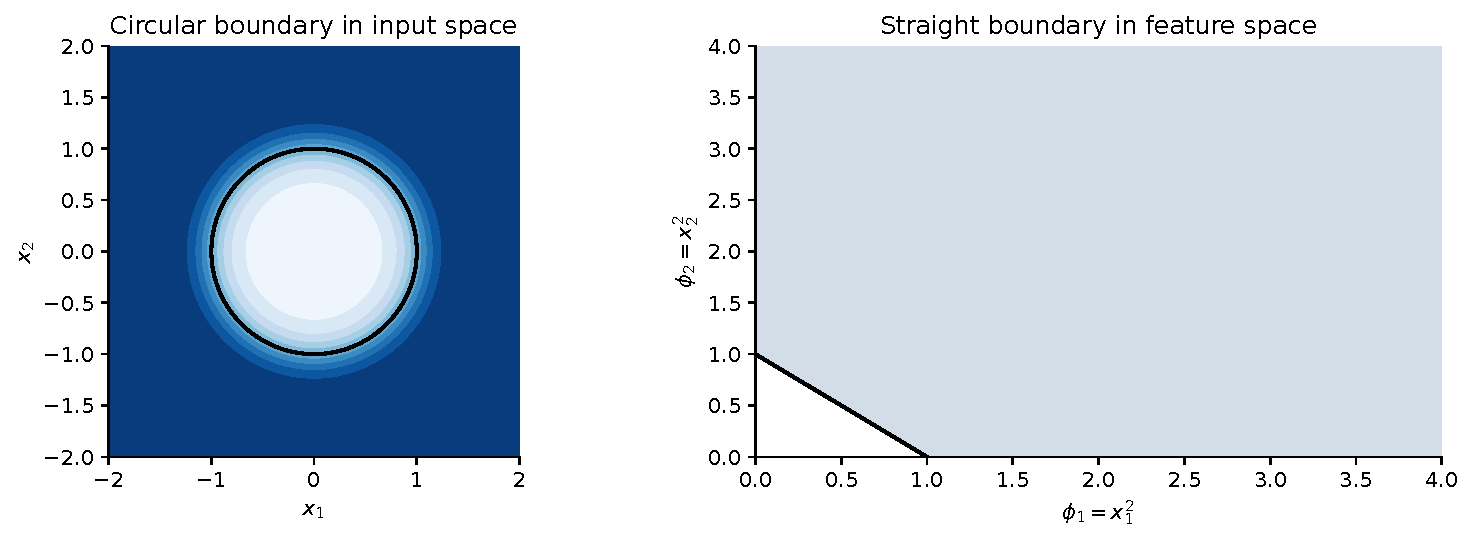
\includegraphics[width=\linewidth]{logreg_1_1/nonlinear_features.pdf}
\caption{One model viewed in two coordinate systems. The curved boundary in
input space becomes straight after the fixed feature transformation. Only the
nonnegative quadrant is reachable in this feature space.}
\end{figure}

\subsection{From a probability model to the likelihood of an observation}
Once an input $x$ is fixed, a Bernoulli model assigns
\[
p_w(Y=y\mid x)=
\begin{cases}p_w(x),&y=1,\\1-p_w(x),&y=0.\end{cases}
\]
Because $y$ is binary, the two cases can be encoded as
\begin{equation}
p_w(Y=y\mid x)=p_w(x)^y\bigl(1-p_w(x)\bigr)^{1-y}.
\label{eq:lr11-bernoulli}
\end{equation}
Check both values: when $y=1$, the second exponent is zero; when $y=0$, the first
is zero. The formula does not make the label continuous. It uses the label as a
selector of the probability assigned to the observed event.

\paragraph{Probability versus likelihood.}
With $w$ fixed, this expression is a probability distribution over $y$; its two
values sum to one. After observing $(x,y)$, the very same expression viewed as a
function of $w$ is a \emph{likelihood}. It asks which parameter choices would
make the observed outcome plausible. It is not a probability distribution over
$w$ and need not integrate to one over parameter space. A Bayesian posterior over
$w$ would additionally require a prior and normalization.

For example, if a grasp succeeds, a model predicting $p=0.9$ assigns likelihood
$0.9$, while one predicting $p=0.2$ assigns $0.2$. If that grasp fails, the
likelihoods reverse their preference: $0.1$ versus $0.8$. A model is judged by
what it said about the event that happened, not just by the thresholded class.

\subsection{Deriving the training objective from maximum likelihood}
Let $\mathcal D=\{(x_n,y_n)\}_{n=1}^N$ and $p_n=p_w(x_n)$. Assume the labels are
conditionally independent across observations given their inputs and the common
parameter $w$. An i.i.d. sample of pairs is a familiar sufficient setup. Then
\[
\mathcal L(w;\mathcal D)=\prod_{n=1}^N
p_n^{y_n}(1-p_n)^{1-y_n}.
\]
The product is a joint conditional probability of the observed labels. Adjacent
video frames or repeated trials on the same object can violate the independence
assumption. The sum loss can still be used as an objective in that case, but the
simple independent-data likelihood interpretation and effective sample size need
care.

We maximize this likelihood. Since $\log$ is strictly increasing, it preserves
which positive value is largest. Since $\log(ab)=\log a+\log b$, it converts
products into sums:
\begin{align*}
\argmax_w\mathcal L(w;\mathcal D)
&=\argmax_w\log\mathcal L(w;\mathcal D)\\
&=\argmax_w\sum_{n=1}^N
\bigl[y_n\log p_n+(1-y_n)\log(1-p_n)\bigr]\\
&=\argmin_w\left\{-\frac1N\sum_{n=1}^N
\bigl[y_n\log p_n+(1-y_n)\log(1-p_n)\bigr]\right\}.
\end{align*}
Negation turns maximization into minimization. Dividing by positive $N$ does not
change the minimizers; it expresses an average per observation. It does change
gradient magnitudes, so the same numerical learning rate need not behave the
same for sum and mean losses.

\begin{definition}[Binary cross-entropy]
For one observation,
\begin{equation}
\boxed{\ell(p,y)=-y\log p-(1-y)\log(1-p).}
\label{eq:lr11-bce}
\end{equation}
For a dataset, the mean negative log-likelihood is
\begin{equation}
\boxed{J(w)=\frac1N\sum_{n=1}^N\ell(p_w(x_n),y_n).}
\label{eq:lr11-mean}
\end{equation}
All logarithms in this section are natural, so losses are measured in nats.
\end{definition}

The brackets in \eqref{eq:lr11-mean} matter: the minus sign applies to both
label-dependent log terms. Changing the logarithm base only multiplies the
objective by a positive constant, leaving its minimizers unchanged.

\subsection{Why a logarithmic penalty makes sense}
The quantity $-\log r$ measures the \emph{surprise} of an event to which the model
assigned probability $r$. An event assigned probability one produces no surprise;
an event assigned a tiny probability produces a large surprise. For independent
events, surprise adds because their probabilities multiply. This is why the
negative logarithm is so natural for a joint probability objective.

\begin{center}
\begin{tabular}{rrrr}
\toprule
Probability of observed outcome $r$ & $0.9$ & $0.5$ & $0.01$\\
\midrule
Surprise $-\log r$ & $0.1054$ & $0.6931$ & $4.6052$\\
\bottomrule
\end{tabular}
\end{center}

For $y=1$, $\ell=-\log p$ decreases as $p$ increases, and
$\partial\ell/\partial p=-1/p$. For $y=0$, $\ell=-\log(1-p)$ increases with $p$,
and $\partial\ell/\partial p=1/(1-p)$. A confidently wrong prediction is much
more expensive than an uncertain one. Correct classification alone does not
make the loss zero: $p=0.51$ and $p=0.99$ both predict one, but their losses for
$y=1$ are about $0.673$ and $0.010$.

\begin{figure}[htbp]
\centering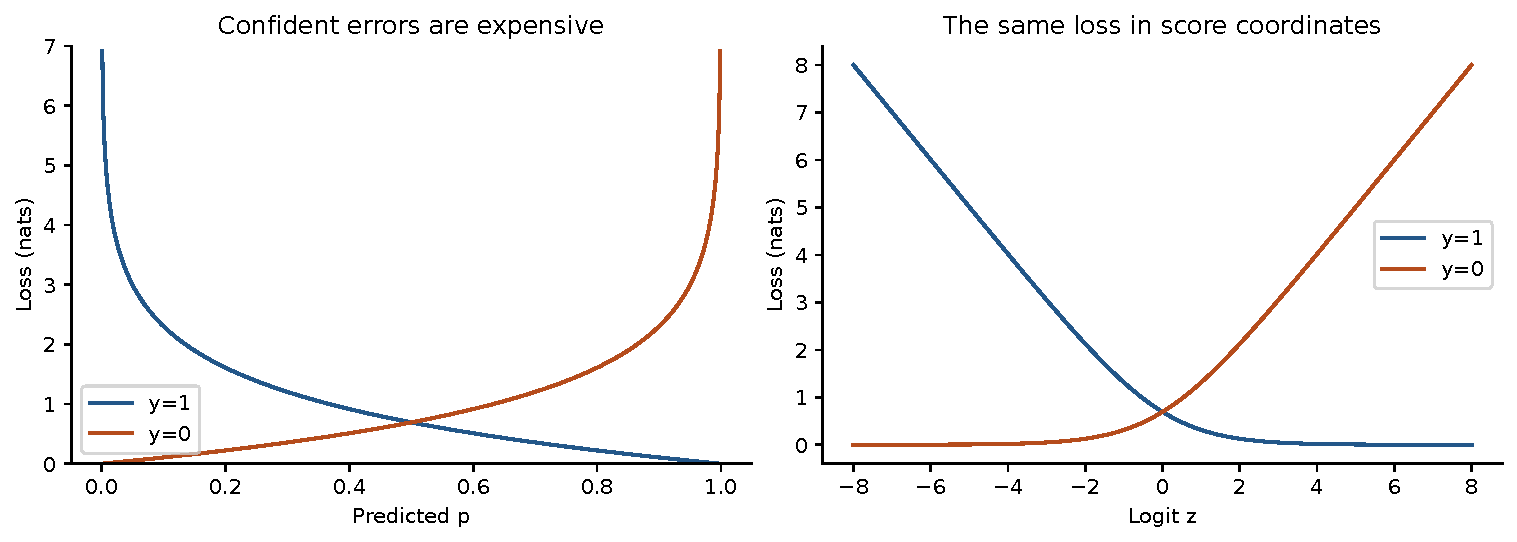
\includegraphics[width=\linewidth]{logreg_1_1/bce.pdf}
\caption{Cross-entropy in probability coordinates (left) and logit coordinates
(right). The probability loss diverges at a wrong endpoint. In logit coordinates
the wrong-direction loss grows approximately linearly for large magnitude.}
\end{figure}

\paragraph{The lecture's two-prediction question.}
For labels $(0,1)$, prediction $(1,1)$ assigns zero joint probability to the
observed data. Its mean BCE is infinite, because the first observation has
$-\log(1-1)=+\infty$. Prediction $(0.5,0.5)$ assigns joint probability $0.25$,
and its mean loss is $-\tfrac12\log(0.25)=\log2\approx0.6931$.
Cross-entropy therefore prefers the second prediction. Exact endpoints are not
produced by a finite mathematical logit, but can occur through rounding. With
$(1-\varepsilon,1-\varepsilon)$ instead, the mean loss is
$-\tfrac12\log[\varepsilon(1-\varepsilon)]$, which diverges as
$\varepsilon\downarrow0$. At an endpoint, interpret zero-weight log terms by
limits; do not compute $0\log0$ directly in floating-point code.

\subsection{Why the best probability is honest, not always extreme}
For a single observed positive label the loss prefers $p\to1$. Does this mean
training should always produce extreme probabilities? Consider repeated outcomes
at the same input with true success probability $q$. The \emph{expected} loss of
reporting $p$ is
\[
r(p;q)=-q\log p-(1-q)\log(1-p).
\]
For $0<q<1$,
\[
\frac{\partial r}{\partial p}
=-\frac{q}{p}+\frac{1-q}{1-p}
=\frac{p-q}{p(1-p)}.
\]
It is negative for $p<q$, zero for $p=q$, and positive for $p>q$. Hence the unique
minimum is the true conditional probability $p=q$. For $q=0$ or $1$, the minimum
is at the corresponding endpoint, approached as a limit by finite logits.
This property is called a \emph{strictly proper scoring rule}.

Suppose ten otherwise identical conditions yield seven successes and three
failures. Their mean loss is $-0.7\log p-0.3\log(1-p)$, minimized at $p=0.7$,
with logit $\log(7/3)\approx0.8473$. Memorizing the latest outcome is not the same
as modeling the underlying probability.

The irreducible minimum is
$r(q;q)=H(q)$, and the excess expected loss is
\[
r(p;q)-H(q)
=q\log\frac{q}{p}+(1-q)\log\frac{1-q}{1-p}
=D_{\mathrm{KL}}\bigl(\operatorname{Bern}(q)\,\|\,
\operatorname{Bern}(p)\bigr)\geq0.
\]
The nonnegativity also follows from the minimization just proved. This gives a
bridge to Section 1.2: cross-entropy is entropy plus the cost of using the wrong
probabilities. A one-hot observed label is an empirical point mass, whose
cross-entropy with the model is precisely the single-observation negative
log-likelihood.

\begin{figure}[htbp]
\centering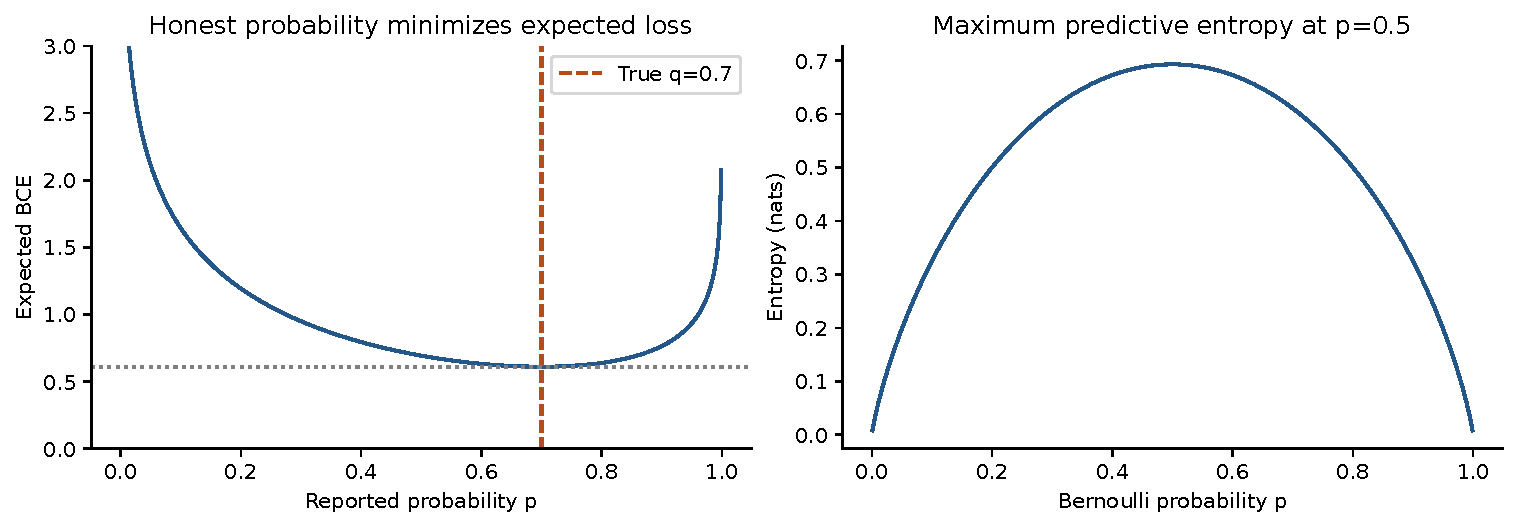
\includegraphics[width=\linewidth]{logreg_1_1/probability_meaning.pdf}
\caption{Left: when the true success frequency is $0.7$, reporting $0.7$ minimizes
expected loss. The dotted horizontal line is the irreducible entropy. Right:
entropy peaks at $0.5$, quantifying uncertainty in a Bernoulli prediction.}
\end{figure}

\paragraph{Empirical versus population risk.}
Training minimizes a sample average. The quantity we ultimately care about is
\[
R(w)=\mathbb E_{X,Y}[\ell(p_w(X),Y)]
=\mathbb E_X\!\left[-q(X)\log p_w(X)
-(1-q(X))\log(1-p_w(X))\right].
\]
This follows by first averaging over the two values of $Y$ at each fixed $X$,
then averaging over inputs. The weights are fixed while this expectation is
evaluated; they vary when comparing models during optimization. Finite data,
misspecified affine log-odds, and distribution shift can keep $p_w$ far from $q$.
A proper loss encourages honest probabilities in the population; it does not
promise that every fitted finite-sample model is calibrated.

\subsection{Deriving the gradient: why the residual is \texorpdfstring{$p-y$}{p-y}}
We want to adjust each weight in the direction that reduces the mean loss.
For one observation, apply the chain rule through $w\to z\to p\to\ell$:
\begin{align*}
\frac{\partial\ell}{\partial p}
&=-\frac{y}{p}+\frac{1-y}{1-p}
=\frac{p-y}{p(1-p)},\\
\frac{\partial p}{\partial z}&=p(1-p),\\
\frac{\partial\ell}{\partial z}&=p-y,\\
\frac{\partial z}{\partial w_j}&=\tilde x_j,\qquad
\boxed{\frac{\partial\ell}{\partial w_j}=(p-y)\tilde x_j.}
\end{align*}
The apparent complicated fractions cancel because of the sigmoid--Bernoulli
pairing. In particular, even when a confidently wrong sigmoid saturates, the
BCE gradient with respect to its logit does not vanish: it approaches $-1$ for
a very wrong positive label and $+1$ for a very wrong negative label.

For $y=1$ and $p=0.2$, $p-y=-0.8$. Gradient descent increases the score in the
direction of this input, making the observed success more probable. More
precisely, for a single-sample update $w^+=w-\eta(p-y)\tilde x$,
\[
z^+=(w^+)^\top\tilde x
=z+\eta(y-p)\|\tilde x\|^2.
\]
For a positive label this increases its score; for a negative label it decreases
it. Other examples may pull in conflicting directions, which is why learning
requires a compromise rather than independent adjustments to every prediction.

\paragraph{Matrix form and dimensions.}
Let $X\in\mathbb R^{N\times(d+1)}$ have row $n$ equal to $\tilde x_n^\top$,
and let $y,p,z\in\mathbb R^N$. Then
\[
z=Xw,\qquad p=\sigma(z)\quad\text{elementwise},\qquad
\boxed{\nabla J(w)=\frac1N X^\top(p-y).}
\]
The gradient has shape $(d+1)$: $(d+1)\times N$ times $N\times1$.
The bias gradient is $N^{-1}\sum_n(p_n-y_n)$ because column zero of $X$ is one.
A full-batch update is
\[
w_{t+1}=w_t-\eta\frac1N X^\top\bigl(\sigma(Xw_t)-y\bigr).
\]
All predictions in this update are evaluated at the \emph{current} weights
$w_t$. Predictions change after the update. For a uniformly sampled minibatch
of size $B$, replace the full average by its batch average. This is an unbiased
estimator of the empirical gradient under uniform sampling. SGD is one possible
solver, not part of the definition of logistic regression.

\paragraph{One complete update by hand.}
Take two observations $x^{(1)}=(0,0),y_1=0$ and
$x^{(2)}=(1,2),y_2=1$, and initialize all three weights to zero. Both
probabilities are $0.5$, so
\[
X=\begin{bmatrix}1&0&0\\1&1&2\end{bmatrix},\quad
p-y=\begin{bmatrix}0.5\\-0.5\end{bmatrix},\quad
\nabla J=\begin{bmatrix}0\\-0.25\\-0.5\end{bmatrix}.
\]
With $\eta=1$, $w^+=(0,0.25,0.5)^\top$. The scores become $(0,1.25)$ and the
probabilities $(0.5,0.7773)$. The mean loss decreases from $0.6931$ to
$\tfrac12[0.6931+\log(1+e^{-1.25})]\approx0.4725$.
This separable toy dataset has no finite unregularized optimum; it illustrates
an update, not convergence to finite weights.

\subsection{Convexity: a proof, and what it does not promise}
Differentiate the gradient again. Since $\partial p_n/\partial w
=p_n(1-p_n)\tilde x_n$,
\begin{equation}
\nabla^2J(w)=\frac1N X^\top D X,\qquad
D=\operatorname{diag}\bigl(p_n(1-p_n)\bigr).
\label{eq:lr11-hessian}
\end{equation}
For any $v\in\mathbb R^{d+1}$,
\[
v^\top\nabla^2J(w)v
=\frac1N\sum_{n=1}^N p_n(1-p_n)(\tilde x_n^\top v)^2\geq0.
\]
Thus the Hessian is positive semidefinite and $J$ is convex in $w$.
Every finite local minimum is global. This proof still works for any \emph{fixed}
nonlinear feature map, since its design matrix remains fixed. It does not establish
convexity for a multilayer network whose feature representation is trained too.

For finite logits, all diagonal entries of $D$ are positive. If $X$ has full
column rank, the Hessian is positive definite and $J$ is strictly convex at every
finite $w$, giving at most one finite minimizer. If columns are redundant, there
may be whole flat directions. Strict convexity does not by itself guarantee
that a minimum is attained.

\paragraph{The separability trap.}
Write $t_n=2y_n-1\in\{-1,1\}$. If some $v$ strictly separates all training
examples, $t_n\tilde x_n^\top v>0$ for every $n$, then
\[
J(cv)=\frac1N\sum_n\log\bigl(1+e^{-c t_n\tilde x_n^\top v}\bigr)
\longrightarrow0\quad(c\to\infty).
\]
For any finite weights each term is strictly positive. The loss has infimum
zero but no finite minimizer. Classification can become perfect while weight
norms keep increasing. Quasi-separation creates related nonexistence issues.
Therefore ``convex'' is not equivalent to ``a unique finite solution exists.''

A common remedy is an $L^2$ penalty on slopes,
\[
J_\lambda(w)=J(w)+\frac\lambda2\|a\|_2^2,\qquad
\nabla J_\lambda=\nabla J+\lambda(0,a^\top)^\top.
\]
It discourages arbitrarily steep confidence transitions. With both classes
present and fixed finite features, penalizing all slopes with $\lambda>0$ also
controls the unpenalized intercept and gives a finite unique optimum. If every
label is one class, an unpenalized bias can still diverge. Penalizing all
coordinates, including the bias, makes the objective coercive and strongly
convex for $\lambda>0$, guaranteeing a unique finite minimizer. The penalty
changes the estimation objective: it is no longer unregularized maximum
likelihood. Its strength must be interpreted relative to sum versus mean loss.

\paragraph{Choosing a learning rate from curvature.}
Because $p_n(1-p_n)\leq1/4$,
\[
0\preceq\nabla^2J(w)\preceq\frac1{4N}X^\top X,\qquad
L=\frac{\|X\|_2^2}{4N}
\]
is a global gradient-Lipschitz bound (spectral norm). Smoothness gives
\[
J(w-\eta g)\leq J(w)-\eta(1-L\eta/2)\|g\|^2,
\qquad g=\nabla J(w).
\]
Thus $0<\eta<2/L$ yields descent when $g\ne0$; $\eta\leq1/L$ is a convenient
conservative choice. Add $\lambda$ to the bound for the stated $L^2$ penalty.
This full-batch bound does not mean every stochastic step decreases the loss.
Standardizing feature scales often improves conditioning and makes the
optimization more efficient.

\begin{figure}[htbp]
\centering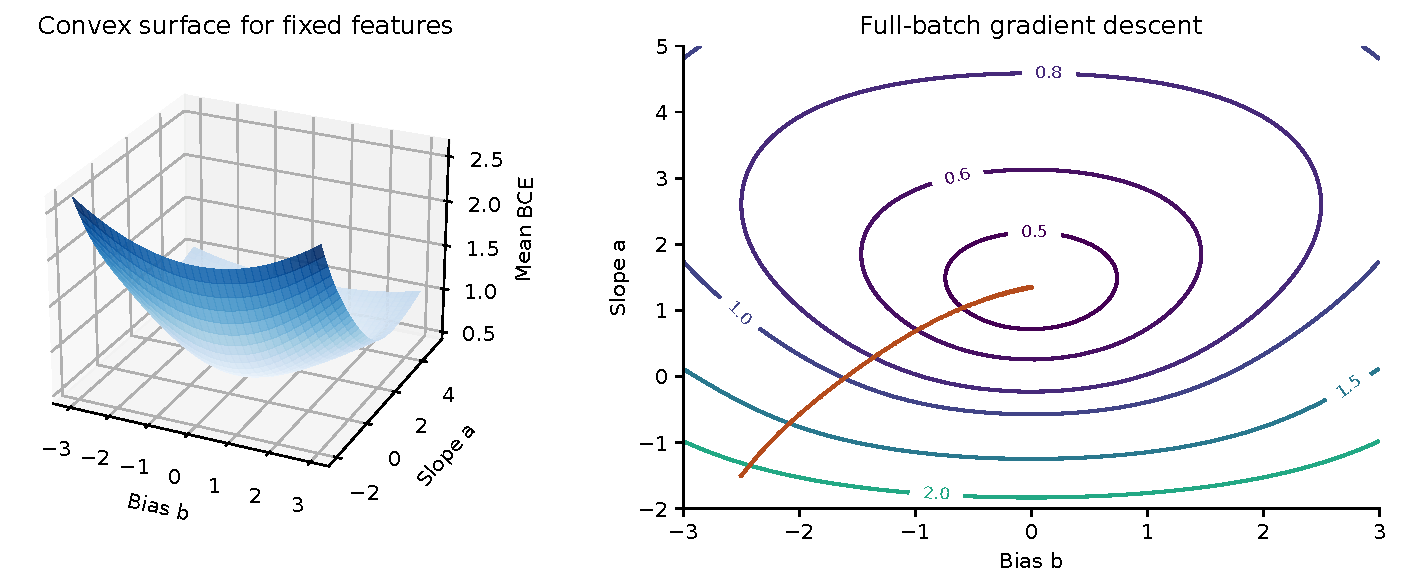
\includegraphics[width=\linewidth]{logreg_1_1/optimization.pdf}
\caption{Mean BCE for a nonseparable one-feature dataset, with bias and slope as
the two axes. The contour plot shows gradient descent from $(-2.5,-1.5)$.
The surface and the contours describe the same objective in parameter space,
not the decision boundary in input space.}
\end{figure}

\subsection{Computational complexity: what exactly is being computed?}
For dense data with $N$ observations and $d$ raw features:
\begin{center}
\begin{tabular}{lll}
\toprule
Operation & Output & Time \\
\midrule
Augmented matrix--vector product $Xw$ & $N$ logits & $\Theta(N(d+1))$ \\
Elementwise sigmoid & $N$ probabilities & $\Theta(N)$ \\
Loss terms and reduction, given logits & One scalar & $\Theta(N)$ \\
Gradient product $X^\top(p-y)$ & $d+1$ derivatives & $\Theta(N(d+1))$ \\
\bottomrule
\end{tabular}
\end{center}
So computing BCE \emph{from raw inputs and weights} is $\Theta(Nd)$ for $d\geq1$.
If probabilities have already been computed and the question only counts the
loss reduction, it is $\Theta(N)$. A full-batch gradient step is also
$\Theta(Nd)$; $T$ steps cost $\Theta(TNd)$. We treat scalar arithmetic and
transcendental functions as constant-cost operations in this usual model.

Storing dense $X$ costs $\Theta(Nd)$ memory, and vectorized predictions need
$\Theta(N)$ additional memory. Minibatches can reduce the working prediction
storage to $\Theta(B)$; streaming avoids storing the full dataset. Sparse matrix
products can cost $\Theta(\operatorname{nnz}(X)+N)$ instead. Explicitly forming
a dense Hessian costs $O(Nd^2)$ time and $O(d^2)$ extra space, which explains why
first-order methods are attractive when $d$ is large.

\subsection{Numerical stability: evaluate the mathematical quantity safely}
The direct expression $-y\log\sigma(z)-(1-y)\log(1-\sigma(z))$ is fragile in
floating point. A large positive score can round $\sigma(z)$ to one, and then
$\log(1-p)$ becomes $\log0$. Large negative scores can overflow $e^{-z}$.
These are numerical failures, not infinite mathematical losses at finite $z$.

Use identities before computing. Since
\[
\log\sigma(z)=z-\log(1+e^z),\qquad
\log(1-\sigma(z))=-\log(1+e^z),
\]
substitution into BCE yields
\begin{equation}
\ell(z,y)=\log(1+e^z)-yz
=\operatorname{softplus}(z)-yz.
\label{eq:lr11-softplus}
\end{equation}
A stable softplus is
$\max(z,0)+\log(1+e^{-|z|})$. For binary labels an even cleaner form is
\[
\boxed{\ell(z,y)=\log\bigl(1+e^{(1-2y)z}\bigr)
=\operatorname{softplus}(-t z),\quad t=2y-1.}
\]
The scalar $tz$ is the signed margin: a large positive margin means confidently
correct, a negative margin means wrong. NumPy's \texttt{logaddexp(0, u)} computes
$\log(1+e^u)$ stably. The signed-margin form also avoids subtracting two large
nearly equal numbers for a correctly classified positive example.

\begin{lstlisting}
import numpy as np

def sigmoid(z):
    z = np.asarray(z, dtype=float)
    return np.exp(-np.logaddexp(0.0, -z))

def loss_and_gradient(X, y, w):
    # X: (N, d+1), y: (N,), w: (d+1,)
    z = X @ w
    loss = np.logaddexp(0.0, (1.0 - 2.0*y)*z).mean()
    gradient = X.T @ (sigmoid(z) - y) / len(y)
    return loss, gradient
\end{lstlisting}

At $z=-1000,y=1$, the loss is approximately $1000$, not a NaN. Clipping
probabilities to $[\varepsilon,1-\varepsilon]$ can prevent a log failure, but
changes the objective near endpoints and can make a stated gradient inconsistent
with that clipped objective. Computing from logits is preferable when available.
Keep $y$ one-dimensional with the code above: mixing shape $(N,1)$ labels and
$(N,)$ probabilities can accidentally broadcast to an $(N,N)$ array.

\subsection{Worked robotics setup: grasp success, cost, and evaluation}
We now connect the equations to an entire modeling workflow. Suppose a robot
uses two nonnegative measurements: centering error $e$ in millimeters and angular
error $\theta$ in degrees. For an interpretable synthetic example, assume the
true conditional success probability is
\begin{equation}
q(e,\theta)=\sigma(3-0.25e-0.08\theta).
\label{eq:lr11-robot}
\end{equation}
These coefficients are illustrative, not measured hardware parameters. Real
success also depends on object geometry, friction, contact, and perception.
The model says that one extra millimeter multiplies success odds by
$e^{-0.25}\approx0.779$, while one extra degree multiplies them by
$e^{-0.08}\approx0.923$, holding the other feature fixed.

At $e=4,\theta=10$, the logit is $1.2$ and $q\approx0.7685$. At
$e=8,\theta=20$, it is $-0.6$ and $q\approx0.3543$. With equal error costs, the
success boundary is
\[
0.25e+0.08\theta=3.
\]
This line is a contour of equal probability, not a physical law of grasping.

\paragraph{Derive the action threshold from consequences.}
Suppose accepting a grasp that fails costs $C_{\mathrm{FP}}$, while rejecting a
grasp that would succeed costs $C_{\mathrm{FN}}$. Assume the two correct decisions
have zero cost. Given a success probability $p$, the expected costs are
\[
\text{accept: }C_{\mathrm{FP}}(1-p),\qquad
\text{reject: }C_{\mathrm{FN}}p.
\]
Accept if the first is smaller, giving
\begin{equation}
p\geq\tau=\frac{C_{\mathrm{FP}}}{C_{\mathrm{FP}}+C_{\mathrm{FN}}},\qquad
z\geq\log\frac{\tau}{1-\tau}.
\label{eq:lr11-cost}
\end{equation}
With $C_{\mathrm{FP}}=8$ and $C_{\mathrm{FN}}=1$, $\tau=8/9\approx0.8889$
and the score threshold is $\log8\approx2.0794$. Equation~\eqref{eq:lr11-robot}
then permits acceptance only when
\[
0.25e+0.08\theta\leq3-\log8\approx0.9206.
\]
The earlier $0.7685$ example would pass a $0.5$ rule but fail this cost-sensitive
rule. The probability model has not changed; the action criterion has.
In deployment this rule relies on useful probability estimates and appropriate
costs. It is not a safety guarantee.

\paragraph{A complete reproducible experiment.}
The companion script generates 1,200 trials using seed 7, with independent
$e\sim U(0,20)$, $\theta\sim U(0,40)$ and
$Y\mid e,\theta\sim\operatorname{Bern}(q(e,\theta))$. It randomly splits them
into 720 training, 240 validation, and 240 test observations. This random split
is appropriate for this independently generated simulation. On real robot
logs, split by object, session, or time as appropriate so near-duplicate frames
and trials do not leak across sets.

Compute each feature's mean $\mu_j$ and standard deviation $s_j$ on the training
set only. Transform all sets using $u_j=(x_j-\mu_j)/s_j$ and prepend the bias
column. Fit the standardized logistic model using full-batch gradient descent
and a fixed illustrative slope penalty $\lambda=0.02$. The script uses the
curvature bound above to choose a conservative step size, with 1,800 updates.
A practical study would select the penalty using validation data too.

Standardization changes coordinates, not the expressive family. If the learned
score is $b_s+\sum_j a_{s,j}(x_j-\mu_j)/s_j$, its physical-unit coefficients are
\[
a_j=\frac{a_{s,j}}{s_j},\qquad
b=b_s-\sum_j\frac{a_{s,j}\mu_j}{s_j}.
\]
However, an $L^2$ penalty in standardized coordinates does change the implicit
penalty on physical-unit coefficients. This is one reason scaling is a modeling
choice as well as a numerical convenience.

\begin{figure}[htbp]
\centering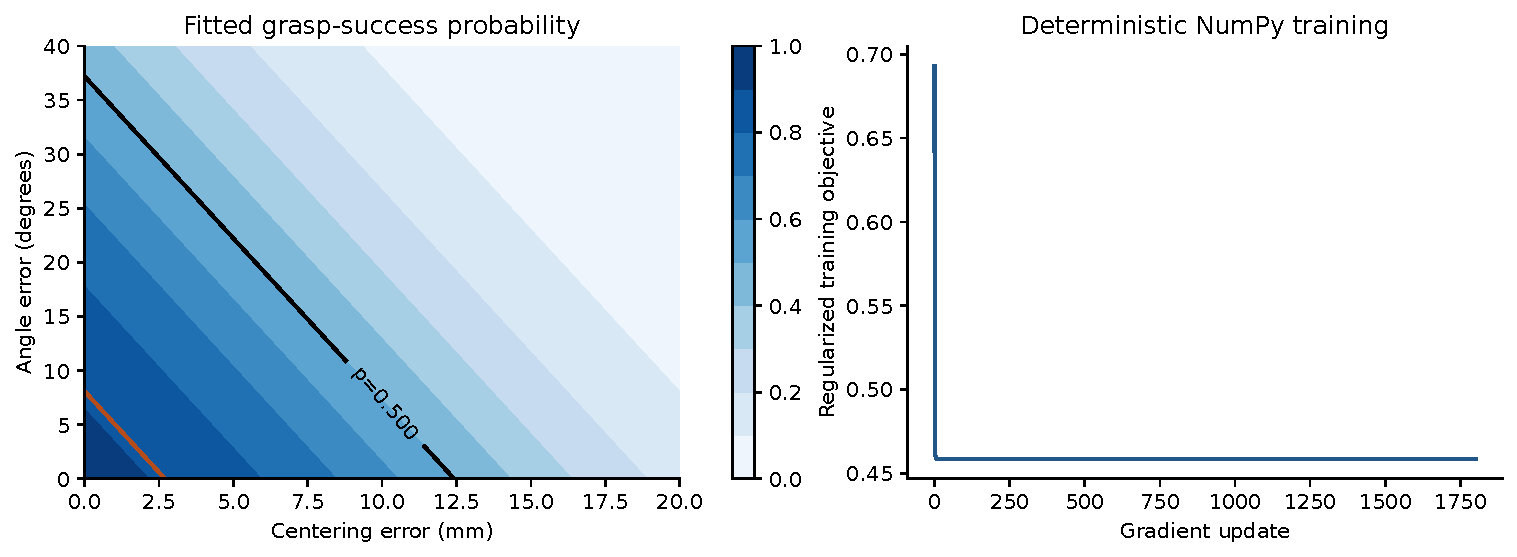
\includegraphics[width=\linewidth]{logreg_1_1/robot_grasp.pdf}
\caption{Synthetic robot experiment. Left: the fitted success field in physical
units, with the $0.5$ and $8/9$ thresholds. Right: the regularized training
objective decreases under the chosen full-batch step size.}
\end{figure}

\paragraph{Evaluate probabilities and decisions separately.}
Report unpenalized test BCE to measure probability quality, accuracy for a stated
threshold, and empirical decision cost for the actual action criterion.
A reliability diagram groups predicted probabilities into bins and compares
each bin's mean probability with its observed success frequency. Small bins are
noisy; an apparent deviation from the diagonal is not automatically systematic
miscalibration. The script records each bin's sample count.

The script also selects a threshold from $0.05,0.06,\ldots,0.95$ using validation
cost alone, then evaluates it on the test data. An empirically selected threshold
can differ from $8/9$ because of finite samples and imperfect probabilities.
Do not select it by looking at test results: the test set is for the final
assessment. For this seeded run the unpenalized test BCE is $0.4317$ nats and accuracy
at $0.5$ is $80.0\%$. The validation-selected threshold is $0.84$.
\begin{center}
\begin{tabular}{lr}
\toprule
Decision threshold & Mean test cost \\
\midrule
$0.5$ & $0.7542$ \\
$8/9$ (cost-derived) & $0.3250$ \\
$0.84$ (validation-selected) & $0.3708$ \\
\bottomrule
\end{tabular}
\end{center}
Here validation tuning does not beat the cost-derived threshold on the test
sample. This is a useful reminder that selecting a threshold on a finite
validation set is itself an estimation problem.
The full numerical output is in the adjacent \texttt{results.json};
all reported quantities can be regenerated from the code.

\begin{figure}[htbp]
\centering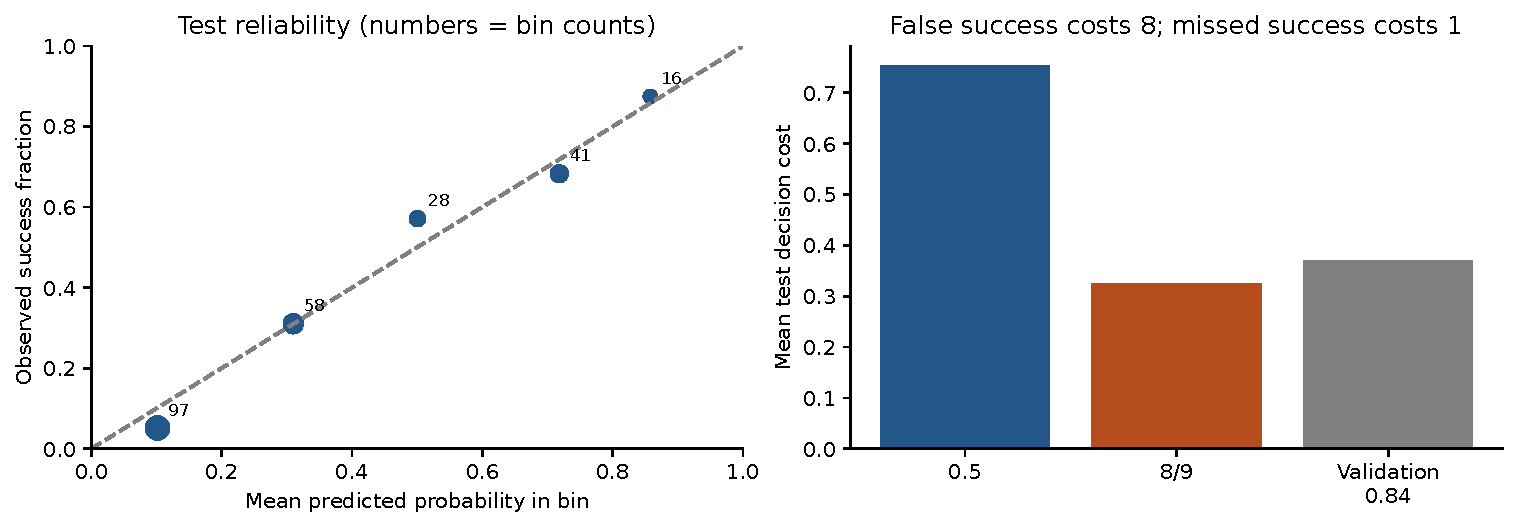
\includegraphics[width=\linewidth]{logreg_1_1/evaluation.pdf}
\caption{Held-out assessment for synthetic grasp trials. Left: a reliability
diagram, with counts showing how much evidence supports each bin. Right: mean
cost at a default threshold, the analytically derived cost threshold, and a
validation-selected threshold. These are one simulation's measurements, not
claims of general superiority or hardware performance.}
\end{figure}

\paragraph{What would break this setup?}
A new gripper or different object material can change $q(x)$ even when the two
features look familiar. Missing interactions may make affine log-odds inadequate.
Selection bias arises if training only records grasps the old policy chose to
attempt; rejected grasps may have no observed outcome. Label errors, rare
failures, correlated trials, and feature drift also matter. More confident
numbers alone solve none of these problems. The model's meaning is conditional
on its observations, data collection, and deployment distribution.

\subsection{From-scratch practice and checks}
The executable companion is
\texttt{deep\_learning/code/logreg\_1\_1.py}. It uses NumPy for the model and
optimization, and Matplotlib for figures; it uses no machine-learning library.
Run it from the repository root:
\begin{lstlisting}[language=bash]
python deep_learning/code/logreg_1_1.py
make dl
\end{lstlisting}
It regenerates seven vector-PDF figures and a JSON result summary in
\path{deep_learning/figures/logreg_1_1/}. The chapter can be compiled with
the committed figures without running Python. The full script includes an
$L^2$-regularized objective, training, data splitting, standardization, evaluation,
and the following meaningful numerical checks:
\begin{enumerate}
\item Compare the analytic gradient against centered finite differences,
$[J(w+\varepsilon e_j)-J(w-\varepsilon e_j)]/(2\varepsilon)$.
\item Check the Hessian's eigenvalues on a small dataset and verify that the
chosen full-batch updates do not increase the regularized objective.
\item Evaluate extreme logits $\pm1000$ and require finite losses and probabilities.
\item Check $\sigma(0)=1/2$ and $\sigma(-z)=1-\sigma(z)$.
\end{enumerate}
These checks catch implementation mistakes; they do not replace the mathematical
proofs or establish generalization to a robot.

\paragraph{Suggested implementation order.}
First reproduce the two-point hand update using only arrays. Then implement
stable sigmoid and BCE, verify the gradient numerically, add repeated updates,
and plot the training loss. Only after that add standardization, a validation
split, and decision costs. Predict what each change should do before running it.
This makes the code an experiment on the mathematical ideas rather than a recipe.

\subsection{Reasoning exercises}
Try these before reading the worked answers below. They are independent of the
main derivation, so the conceptual narrative need not be interrupted.
\begin{exercise}[Same classes, different probabilities]
For $w=(-3,1,1)^\top$, compare $w$ and $10w$ at $(1,2)$ and $(2,2)$.
Do the boundaries, hard predictions, and losses for a positive label agree?
\end{exercise}
\begin{exercise}[Recover a probability model]
An intercept-only dataset contains 20 successes and 30 failures. Derive the
maximum-likelihood probability and intercept. What happens if all 50 succeed?
\end{exercise}
\begin{exercise}[Costs change a boundary]
A classifier has score $z=-3+x_1+x_2$. Derive the action boundary when a false
positive costs nine times a false negative. Which side predicts one?
\end{exercise}
\begin{exercise}[Feature maps and convexity]
Use features $(x_1,x_2,x_1x_2)$ to express XOR on $\{-1,1\}^2$. Explain why the
training objective is convex in its coefficients, despite the nonlinear boundary.
Would the same proof apply if the features were outputs of a trained hidden layer?
\end{exercise}
\begin{exercise}[Complexity and data shape]
For $N=10^6$ and $d=100$, identify the dominant forward-pass operation. Explain
why storing labels as $(N,1)$ while predictions have shape $(N,)$ is dangerous.
How does a batch of size $B$ change working memory and per-step time?
\end{exercise}

\subsection{Worked answers and conceptual checkpoints}
\paragraph{1. Scaling.}
At $(1,2)$, both logits are zero and both probabilities are $0.5$. At $(2,2)$,
the logits are $1$ and $10$, with probabilities about $0.7311$ and $0.99995$.
Positive-label losses are $\log(1+e^{-1})\approx0.3133$ and
$\log(1+e^{-10})\approx0.0000454$. Boundaries and hard classes agree. If the
label at $(2,2)$ were zero instead, the larger scale would be far more costly:
about $10.00005$ versus $1.3133$. Confidence has consequences.

\paragraph{2. Intercept-only estimation.}
The loss is $-0.4\log p-0.6\log(1-p)$; differentiating gives the minimum
$p=0.4$. Thus $b=\log(0.4/0.6)=\log(2/3)\approx-0.4055$. If all labels are one,
the loss decreases as $b\to+\infty$, and no finite unregularized optimum exists.

\paragraph{3. Costs.}
The threshold is $\tau=9/10$, so the logit threshold is $\log9$. The new boundary
is $x_1+x_2=3+\log9\approx5.1972$, with class one on the greater-than side.
It is parallel to the equal-cost boundary and requires stronger evidence.

\paragraph{4. Fixed features.}
Take zero bias and zero coefficients on $x_1,x_2$, with coefficient $-k$ on
$x_1x_2$, $k>0$. The four signed scores have the required signs. The Hessian
proof applies to the resulting fixed design matrix. With a trainable hidden
layer, the feature matrix itself depends on parameters, and the positive
semidefinite form above is no longer the full Hessian.

\paragraph{5. Computation.}
The dense product $Xw$ uses roughly $N(d+1)$ multiply--accumulate operations,
about $10^8$ here. Broadcasting $(N,)$ minus $(N,1)$ can create an $(N,N)$ array,
which is both mathematically wrong and enormous. A dense batch step costs
$\Theta(Bd)$ time and stores $\Theta(Bd)$ feature entries if batches are streamed,
plus parameters and $\Theta(B)$ temporary predictions. An epoch still processes
$N$ observations and costs $\Theta(Nd)$.

\begin{keyidea}[Reconstruct the method from its meaning]
An affine score describes additive log-odds. The sigmoid converts that evidence
into a Bernoulli probability. Independence turns observed-label probabilities
into a product likelihood, and the negative logarithm turns that product into
an additive loss. The gradient $X^\top(p-y)/N$ adjusts evidence according to
probability errors. Convexity follows from nonnegative Bernoulli variances, but
finite solutions require more than convexity. Finally, the decision threshold
comes from the consequences of actions, not from the probability model alone.
\end{keyidea}

\paragraph{Scope and reading.}
This section expands the supplied lecture excerpts (slides 5--10 and their
questions). Section 1.2 can develop entropy, KL divergence, and maximum likelihood
more generally; the later sections can reinterpret the same affine--sigmoid
computation as a neural-network unit. General background texts already present
in this repository include \citet{bishop2006pattern} and
\citet{goodfellow2016deep}. All plots in this section are generated by its companion
script from explicit formulas or synthetic data.

% Section 1.2: information theory and maximum likelihood from first principles.
\section{Cross Entropy, KL Divergence, and Maximum Likelihood}
\label{sec:logreg_to_mlp:cross_entropy_kl_divergence_and_maximum_likelihood}

\begin{keyidea}[Three quantities and three questions]
Entropy asks: how unpredictable is the source itself? Cross-entropy asks: how
surprised will a particular model be by that source? KL divergence asks: how much
extra surprise does using that model create? Maximum likelihood chooses the
model that assigns the greatest joint probability, or density, to the observed
data. These ideas connect through one operation: averaging negative log
probabilities under the distribution that supplies the observations.
\end{keyidea}

\subsection{Start with a robot that must describe what it sees}
A mobile robot sends a stream of corridor events: clear path, person, cart, or
blocked path. Suppose their long-run probabilities are
\[
P=(1/2,1/4,1/8,1/8).
\]
Sending two bits for every event works: there are four possibilities. But the
outcomes are not equally common. Could we give frequent outcomes shorter messages
and rare ones longer messages, reducing the average communication cost?

Now imagine the robot's model predicts a different frequency distribution $Q$.
Even if the communication channel is perfect, a code designed for $Q$ can be
wasteful on events actually drawn from $P$. This is a concrete way to separate
\emph{unavoidable uncertainty} from \emph{avoidable model mismatch}.
The same distinction applies to prediction: a noisy task can have a positive
best possible log loss, while a confident but wrong model adds further loss.

The narrative in this section is
\[
\text{surprise}\longrightarrow\text{average surprise}\longrightarrow
\text{mismatch}\longrightarrow\text{estimating a model from data}.
\]
We first work on a finite outcome space. Continuous measurements need additional
care and are treated explicitly later. Throughout, $P$ is the distribution that
supplies outcomes and $Q$ is the distribution used to score them, unless an
expression explicitly swaps their roles.

\subsection{Why should information be a negative logarithm?}
Suppose an event has probability $p$. We seek a numerical measure $I(p)$ of the
information gained when learning that it occurred. A plausible set of
requirements is:
\begin{enumerate}
\item A certain event gives no new information: $I(1)=0$.
\item A rarer event is more informative: $I(p)$ decreases as $p$ increases.
\item For independent events, information adds: $I(pq)=I(p)+I(q)$.
\item The measure varies continuously with probability.
\end{enumerate}
The independence clause is essential: probabilities multiply for independent
events. For dependent events, the relevant factorization is
$P(A,B)=P(A)P(B\mid A)$, so information adds using a conditional probability.

To see what these requirements imply, set $p=e^{-t}$ and define
$F(t)=I(e^{-t})$ for $t\geq0$. Then
\[
F(t+s)=F(t)+F(s).
\]
For positive integers, repeated addition gives $F(n)=nF(1)$. Dividing an interval
into equal parts gives $F(m/n)=(m/n)F(1)$ for nonnegative rationals. Continuity
extends this to real $t\geq0$. Therefore $F(t)=ct$, with $c>0$ by the rarity
requirement, and
\[
\boxed{I(p)=-c\ln p.}
\]
The choice of $c$ fixes the unit. With base-two logarithms, a fair coin outcome
has information $-\log_2(1/2)=1$ bit. With natural logarithms the unit is a nat.
Since $\log_2 p=\ln p/\ln2$, a value in nats divided by $\ln2$ is its value in
bits. Information here is about reduction of probabilistic uncertainty, not the
semantic importance of a message. A rare sensor glitch can have high surprise
without being useful for navigation.

\paragraph{One event versus a distribution.}
For $P=(1/2,1/4,1/8,1/8)$, the four event surprises are $1,2,3,3$ bits.
A particular observed event has one of these values. Entropy will be the average
of those values before we know which event will occur. Do not confuse the
information of an outcome with the uncertainty of the whole distribution.

\begin{figure}[htbp]
\centering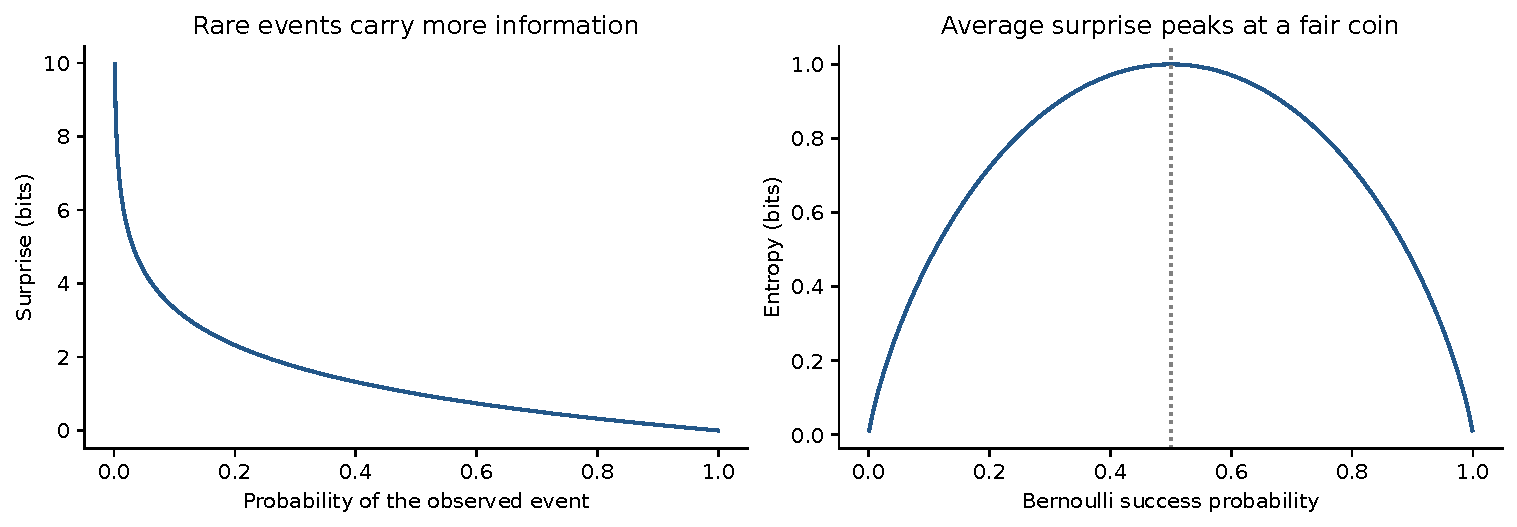
\includegraphics[width=\linewidth]{information_1_2/surprise_entropy.pdf}
\caption{Left: surprise of one event grows as its probability decreases. Right:
the average surprise of a Bernoulli source is largest at equal probabilities.
These curves answer different questions: event surprise and source uncertainty.}
\end{figure}

\subsection{Expectation turns surprise into entropy}
For a finite random variable $X$ with outcomes $x_1,\ldots,x_K$, let
$p_k=P(X=x_k)$. By the definition of expectation, any function $f(X)$ has mean
$\sum_k p_k f(x_k)$. Choosing $f(x)=-\log P(x)$ gives
\begin{equation}
\boxed{H(P)=\mathbb E_{X\sim P}[-\log P(X)]
=-\sum_{k=1}^K p_k\log p_k.}
\label{eq:info12-entropy}
\end{equation}
The weights outside the logarithm describe \emph{how often} an event occurs;
the logarithm describes \emph{how surprising} that event is. Entropy is not
$-\log\mathbb E[P(X)]$, and not an unweighted average over the list of possible
outcomes. Moving a nonlinear logarithm outside an expectation changes the
quantity.

For the robot stream, in bits,
\[
H(P)=\tfrac12(1)+\tfrac14(2)+\tfrac18(3)+\tfrac18(3)=1.75.
\]
This is below the two bits needed by an equiprobable four-outcome source.
A deterministic source has entropy zero: it never surprises an observer who
knows the distribution. On a $K$-outcome space,
\[
0\leq H(P)\leq\log K,
\]
with the upper bound attained by the uniform distribution. We will prove the
upper bound from KL nonnegativity below. Zero-probability events contribute
zero by the continuous extension $\lim_{t\downarrow0}t\log t=0$.

\paragraph{A thought experiment.}
Imagine predicting the next symbol from a fair coin source versus a coin that
comes up heads $99\%$ of the time. For the biased coin, usually there is almost
nothing new to learn, but occasionally a tail is very surprising. Entropy
balances these two facts through a frequency-weighted average. It does not
simply count the number of logically possible outcomes.

\subsection{Coding makes the average operational}
A binary \emph{prefix code} is a collection of bit strings in which no complete
codeword is the prefix of another. This allows concatenated messages to be
decoded without separators. For the robot stream, consider these three codes:
\begin{center}
\begin{tabular}{lrrrr}
\toprule
Event & True $P$ & $P$-matched code & Uniform code & $R$-matched code\\
\midrule
Clear & $1/2$ & 0 & 00 & 110\\
Person & $1/4$ & 10 & 01 & 111\\
Cart & $1/8$ & 110 & 10 & 10\\
Blocked & $1/8$ & 111 & 11 & 0\\
\bottomrule
\end{tabular}
\end{center}
The last code matches $R=(1/8,1/8,1/4,1/2)$. All three are valid prefix codes;
they simply allocate short words differently. Their expected lengths under
$P$ are, respectively,
\[
1.75,\qquad2,\qquad
\tfrac12(3)+\tfrac14(3)+\tfrac18(2)+\tfrac18(1)=2.625\ \text{bits}.
\]
The first code is most efficient for this source. The last makes the common
``clear'' event expensive and saves bits on a rare event instead.

\paragraph{Why ideal lengths are negative log probabilities.}
A complete binary code with lengths $\ell_k$ satisfies
$\sum_k2^{-\ell_k}=1$. Think of each prefix as selecting a fraction
$2^{-\ell_k}$ of the infinite binary tree. Assigning probability $q_k$ the
fraction $q_k$ suggests the ideal length $\ell_k=-\log_2q_k$.
The code tree has only integer depths, however; these ideal lengths need not be
integers. The dyadic probabilities in the table were chosen so they are.

More generally, the Kraft inequality says prefix-code lengths satisfy
$S=\sum_k2^{-\ell_k}\leq1$. Set $r_k=2^{-\ell_k}/S$. Then, in bits,
\[
\mathbb E_P[\ell_X]
=-\sum_kp_k\log_2r_k-\log_2S
=H(P)+D_{\mathrm{KL}}(P\|R)-\log_2S\geq H(P).
\]
This lower bound uses the KL nonnegativity proved shortly. Conversely, choosing
$\ell_k=\lceil-\log_2p_k\rceil$ gives a prefix code with
\[
H(P)\leq\mathbb E_P[\ell_X]<H(P)+1
\]
when the source has positive probabilities on its supported outcomes.
For blocks of $n$ independent events, applying the construction to the block
probabilities gives an overhead of less than one bit \emph{per block}, hence
less than $1/n$ bit per event.

\begin{warning}[Read the slide's coding statement precisely]
Entropy is an ideal average code length and an asymptotically achievable rate
for an i.i.d. source, not necessarily the exact length of a one-symbol binary
code. A Bernoulli source can have entropy $0.2$ bits even though a single
nontrivial binary symbol needs an integer-length codeword. Block coding is how
fractional rates become meaningful. Dependencies require conditional or joint
coding; the marginal entropy alone need not be the best rate for a sequence.
\end{warning}

\subsection{Cross-entropy: keep the source, change the scoring model}
Suppose outcomes still come from $P$, but we evaluate them using probabilities
$q_k=Q(X=x_k)$. The average model-assigned surprise is
\begin{equation}
\boxed{H(P,Q)=\mathbb E_{X\sim P}[-\log Q(X)]
=-\sum_kp_k\log q_k.}
\label{eq:info12-crossentropy}
\end{equation}
The first argument determines the averaging weights. The second determines the
logarithmic score. Swapping the arguments changes both roles. This distinction
is the single most useful way to read a cross-entropy expression.

For the robot source and a uniform model, every event receives two bits of
surprise, so $H(P,Q)=2$. For $R$ above, $H(P,R)=2.625$. In both cases the actual
source remains $P$ and has the same entropy $1.75$.

For a general model $Q$ with positive probability wherever $P$ has positive
probability, the ideal $Q$-based length is $-\log_2q_k$. Rounded Shannon lengths
have expected length between $H(P,Q)$ and $H(P,Q)+1$ bits. This is an ideal or
asymptotic mismatched-coding interpretation; an arbitrary integer code described
as ``optimized for $Q$'' need not have length exactly $-\log_2q_k$.

\paragraph{Support is part of the meaning.}
If $p_k>0$ but $q_k=0$, an event that really can happen has been declared
impossible. Its log loss is infinite, so $H(P,Q)=+\infty$. If $p_k=0$, that
outcome is never scored under $P$ and its term is defined to contribute zero.
Do not evaluate $0\log0$ naively in numerical code.

\begin{figure}[htbp]
\centering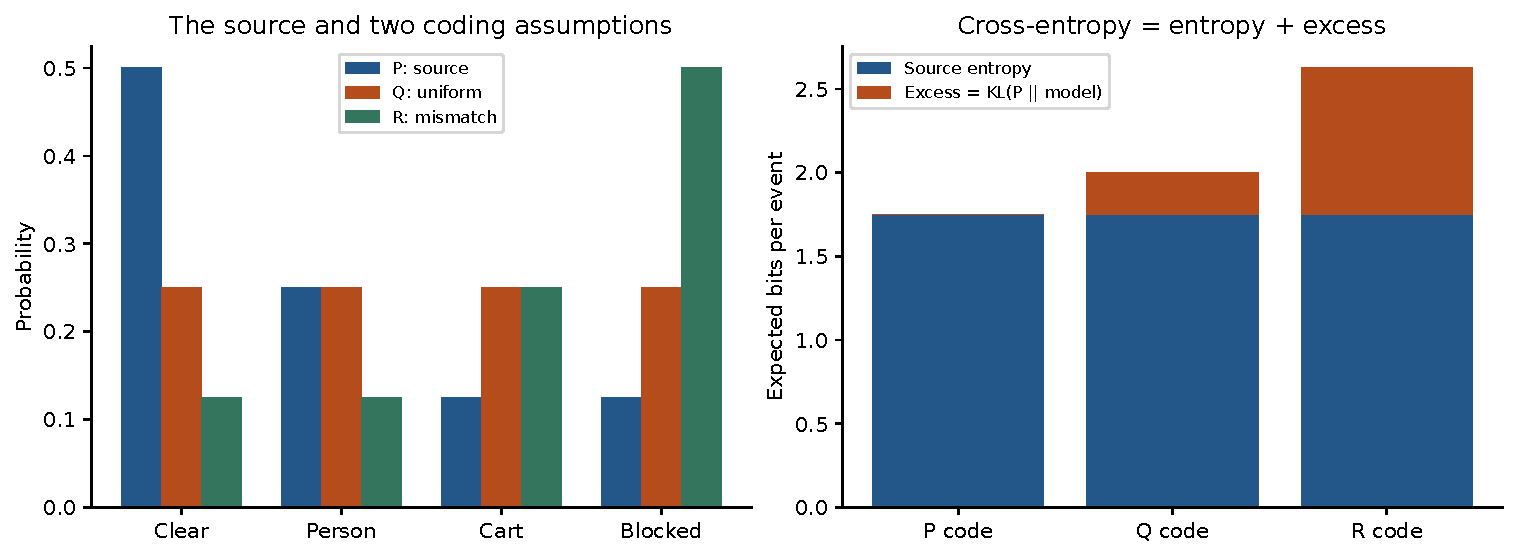
\includegraphics[width=\linewidth]{information_1_2/coding.pdf}
\caption{The same source is scored using three models. The unavoidable source
entropy is unchanged. The additional orange part of each expected code length
is KL divergence. The probabilities are dyadic, so the displayed coding costs
are exact for the prefix codes in the table.}
\end{figure}

\subsection{KL divergence is the excess expected log loss}
Subtract the source entropy from cross-entropy, assuming the expressions are
finite, and collect the logarithms:
\begin{align}
H(P,Q)-H(P)
&=\sum_kp_k\bigl(\log p_k-\log q_k\bigr)\notag\\
&=\sum_kp_k\log\frac{p_k}{q_k}
=\mathbb E_{X\sim P}\!\left[\log\frac{P(X)}{Q(X)}\right]
=:D_{\mathrm{KL}}(P\|Q).
\label{eq:info12-kl}
\end{align}
Equivalently, $D_{\mathrm{KL}}(P\|Q)=-\mathbb E_P\log[Q(X)/P(X)]$,
which matches the slide. Thus
\[
\boxed{H(P,Q)=H(P)+D_{\mathrm{KL}}(P\|Q).}
\]
For infinite quantities, do not treat $+\infty-\infty$ as a legitimate
subtraction; define KL through the log-ratio expression with suitable support
and integrability conditions.

Each individual log ratio may be positive or negative: a model can assign
\emph{more} probability than $P$ to an outcome. KL is the average over $P$.
Normalization forces a tradeoff: giving extra probability to some outcomes
leaves less for others. The average cannot be negative.

\paragraph{Proof of nonnegativity, including zero probabilities.}
The elementary inequality $\log t\leq t-1$ for $t>0$ follows by minimizing
$t-1-\log t$: its derivative is $1-1/t$, and its minimum at $t=1$ is zero.
Let $S=\{k:p_k>0\}$, and first suppose $q_k>0$ on $S$. Applying the inequality
to $t=q_k/p_k$ gives
\begin{align*}
-D_{\mathrm{KL}}(P\|Q)
&=\sum_{k\in S}p_k\log\frac{q_k}{p_k}\\
&\leq\sum_{k\in S}p_k\left(\frac{q_k}{p_k}-1\right)
=\sum_{k\in S}q_k-1\leq0.
\end{align*}
Equality requires $q_k=p_k$ for every $k\in S$ and no probability mass outside
$S$; hence $P=Q$. If $Q$ has a zero on positive $P$ mass, KL is infinite and the
inequality still holds. This proves both nonnegativity and the equality case.

\paragraph{Consequences.}
The best possible predictive distribution under expected log loss is $Q=P$.
Moreover, using the uniform distribution $U_k=1/K$,
\[
D_{\mathrm{KL}}(P\|U)=\sum_kp_k\log p_k+\log K
=\log K-H(P)\geq0,
\]
proving the maximum-entropy bound. An unrestricted distribution family can attain
zero KL; a restricted model family may not contain $P$ and may have a positive
minimum mismatch.

\subsection{Why KL is directed and is not a distance metric}
For a concrete example, use natural logs and
$P=(0.8,0.2)$, $Q=(0.5,0.5)$. Then
\begin{align*}
D_{\mathrm{KL}}(P\|Q)
&=0.8\ln1.6+0.2\ln0.4\approx0.192745,\\
D_{\mathrm{KL}}(Q\|P)
&=0.5\ln0.625+0.5\ln2.5\approx0.223144.
\end{align*}
Different sampling distributions produce different averages. KL is not symmetric
and therefore cannot be a metric; it also does not generally satisfy the
triangle inequality. It is nonnegative and identifies equality, but those two
properties alone do not make a geometric distance.

For an explicit triangle-inequality counterexample, take
$A=(1,0)$, $B=(1/2,1/2)$, and $C=(1/4,3/4)$. Then
$D(A\|C)=\ln4\approx1.3863$, while
$D(A\|B)+D(B\|C)=\ln2+\tfrac12\ln(4/3)\approx0.8370$.
The direct divergence exceeds the sum through the intermediate distribution.

The support asymmetry is even sharper. For $P=(1,0)$ and $Q=(1/2,1/2)$,
$D_{\mathrm{KL}}(P\|Q)=\ln2$, while $D_{\mathrm{KL}}(Q\|P)=+\infty$.
Under $P$ only the first event is sampled. Under $Q$ the second event occurs with
positive probability but is impossible under $P$.

\begin{figure}[htbp]
\centering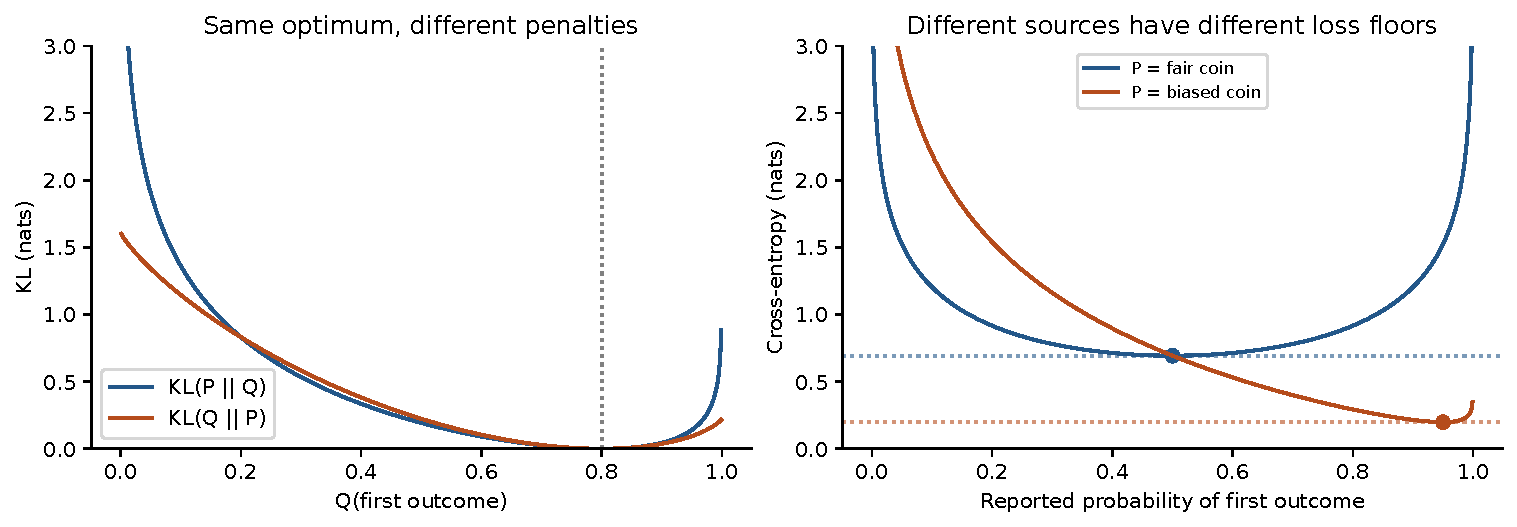
\includegraphics[width=\linewidth]{information_1_2/kl_and_floor.pdf}
\caption{Left: the two directions have the same zero when the distributions
match, but different penalties elsewhere. Right: different true sources have
different minimum cross-entropies. Subtracting each source's entropy isolates
model mismatch. Natural logs are used in both panels.}
\end{figure}

\subsection{Conditioning: knowing the context changes uncertainty}
A robot's observations are not drawn from one label distribution independently
of its inputs. Let $X$ denote the observed context and $Y$ a semantic label.
The relevant uncertainty is the conditional entropy
\[
H_P(Y\mid X)=\mathbb E_{X\sim P_X}
\left[-\sum_y P(y\mid X)\log P(y\mid X)\right].
\]
We average uncertainty \emph{within} each context over how often contexts occur.
Using $P(x,y)=P(x)P(y\mid x)$ and taking negative logs and expectations gives the
chain rule
\[
H_P(X,Y)=H_P(X)+H_P(Y\mid X).
\]
The expected information gained about $Y$ from knowing $X$ is
\[
I_P(X;Y)=H_P(Y)-H_P(Y\mid X)
=D_{\mathrm{KL}}(P_{XY}\|P_XP_Y)\geq0.
\]
This follows by expanding the joint log ratio and collecting the marginal and
conditional terms. Conditioning reduces uncertainty \emph{on average}; a
particular unusual context can have more label entropy than the marginal.

For a conditional model $Q_\theta(y\mid x)$, expected log loss decomposes as
\begin{equation}
\underbrace{\mathbb E_{P_{XY}}[-\log Q_\theta(Y\mid X)]}_{\text{conditional cross-entropy}}
=H_P(Y\mid X)+
\mathbb E_{P_X}D_{\mathrm{KL}}\bigl(P(\cdot\mid X)\|Q_\theta(\cdot\mid X)\bigr).
\label{eq:info12-conditional}
\end{equation}
To derive it, at each fixed $x$ add and subtract
$-\sum_yP(y\mid x)\log P(y\mid x)$, then average over $x$.
This is the version most directly relevant to supervised learning.

\subsection{Maximum likelihood: choosing a model after seeing data}
We now move from two known distributions to an unknown source. Let
$\mathcal D=(x^{(1)},\ldots,x^{(m)})$ be observations drawn independently from a
common but unknown distribution $P_{\mathrm{data}}$. A parametric family
$Q_\theta$ is a set of candidate distributions indexed by $\theta$.

Before observing data, $Q_\theta(x)$ is a probability as a function of $x$ for a
fixed parameter. After observing the data, the same formula, considered as a
function of $\theta$, is a \emph{likelihood}. The data are held fixed while we
compare models:
\[
\mathcal L(\theta;\mathcal D)
=Q_\theta(\mathcal D),\qquad
\hat\theta_{\mathrm{ML}}\in\argmax_\theta\mathcal L(\theta;\mathcal D).
\]
We use membership in the argmax set because a maximizer might not be unique.
There can also be no finite maximizer, as with separable unregularized logistic
regression in Section 1.1. An \emph{estimator} is a rule mapping a dataset to a
parameter value; before sampling, it is itself random. Its realized output is
an estimate.

Likelihood is not a posterior probability of $\theta$. A posterior requires a
prior through Bayes' rule. A high likelihood also does not by itself establish
that the family is correct, or that the estimate will generalize.

\paragraph{Why independence appears in the derivation.}
Under the i.i.d. assumption,
\[
Q_\theta(\mathcal D)=\prod_{i=1}^m Q_\theta(x^{(i)}).
\]
For correlated observations, one instead needs an appropriate joint model, for
example
\[
Q_\theta(x^{(1)})\prod_{i=2}^mQ_\theta(x^{(i)}\mid x^{(1:i-1)}).
\]
The logarithm still turns a product into a sum, but the factors are conditional.
Treating adjacent robot-video frames as independent is a modeling assumption,
not an automatic consequence of having stored them in separate rows.

\subsection{The empirical distribution: turning a dataset into an expectation}
For discrete outcomes, define
\[
\hat P_m(x)=\frac1m\sum_{i=1}^m\mathbf 1\{x^{(i)}=x\}.
\]
It is the observed relative frequency of each outcome. Repeated observations
count repeatedly. For any function $f$,
\begin{align*}
\mathbb E_{\hat P_m}[f(X)]
&=\sum_x\left[\frac1m\sum_i\mathbf1\{x^{(i)}=x\}\right]f(x)\\
&=\frac1m\sum_i\sum_x\mathbf1\{x^{(i)}=x\}f(x)
=\frac1m\sum_i f(x^{(i)}).
\end{align*}
This is why a sample average can be written as an expectation: we have changed
the averaging distribution to the empirical one. It is not an assertion that
$\hat P_m$ equals the unknown true distribution.

For the sequence $(A,A,A,B,C)$, the empirical distribution over $(A,B,C)$ is
$(3/5,1/5,1/5)$, not $(1/3,1/3,1/3)$. If we instead regard the five observation
\emph{indices} as equally likely, each has mass $1/5$; mapping indices to their
values combines the repeated $A$ outcomes. Keeping those spaces distinct avoids
many empirical-entropy mistakes.

\subsection{Every step of the MLE--cross-entropy--KL equivalence}
For a discrete i.i.d. model with probabilities positive on observed outcomes,
\begin{align}
\argmax_\theta Q_\theta(\mathcal D)
&=\argmax_\theta\prod_{i=1}^m Q_\theta(x^{(i)})
&&\text{(independence)}\notag\\
&=\argmax_\theta\sum_{i=1}^m\log Q_\theta(x^{(i)})
&&\text{(monotone log)}\notag\\
&=\argmax_\theta\frac1m\sum_{i=1}^m\log Q_\theta(x^{(i)})
&&\text{(positive scaling)}\notag\\
&=\argmax_\theta\mathbb E_{\hat P_m}\log Q_\theta(X)
&&\text{(empirical mean)}\notag\\
&=\argmin_\theta\mathbb E_{\hat P_m}[-\log Q_\theta(X)]
&&\text{(negation)}\notag\\
&=\argmin_\theta H(\hat P_m,Q_\theta)
&&\text{(definition)}\notag\\
&=\argmin_\theta\{H(\hat P_m,Q_\theta)-H(\hat P_m)\}
&&\text{(constant in $\theta$)}\notag\\
&=\argmin_\theta D_{\mathrm{KL}}(\hat P_m\|Q_\theta).
\label{eq:info12-mlechain}
\end{align}
These are equal sets of optimizers, not equal numerical objectives.
In particular, the sum of log probabilities equals $m$ times the empirical
expectation, not the expectation itself. The factor disappears only because a
positive constant does not change the argmax. Likewise, removing empirical
entropy changes the objective value but not its optimizer or gradient.

\paragraph{Which way does the KL point?}
The empirical distribution comes first: it supplies the data being averaged.
The model comes second: its probabilities are evaluated on those data.
This is forward KL, $D_{\mathrm{KL}}(\hat P_m\|Q_\theta)$, not
$D_{\mathrm{KL}}(Q_\theta\|\hat P_m)$. The order is determined by the likelihood
calculation, not by a freely chosen convention.

\paragraph{Population interpretation.}
If the relevant expectations are finite, the population objective is
\[
\mathbb E_{P_{\mathrm{data}}}[-\log Q_\theta(X)]
=H(P_{\mathrm{data}})+D_{\mathrm{KL}}(P_{\mathrm{data}}\|Q_\theta).
\]
Training substitutes a sample average for this unknown expectation. A law of
large numbers gives convergence for a fixed $\theta$ under suitable assumptions;
consistency of the \emph{optimizer} requires additional conditions, such as
identifiability and control of the objective over the family. Finite-sample
maximum likelihood does not automatically find the true distribution.
If the family is misspecified, even a population-optimal parameter can retain
positive KL.

\subsection{Worked MLEs: Bernoulli and categorical models}
For a Bernoulli model $Q_\theta(1)=\theta$, let $s$ of $m$ labels be one. The
likelihood of the observed ordered sequence is
\[
\mathcal L(\theta)=\theta^s(1-\theta)^{m-s}.
\]
If only the count is observed, its binomial probability includes
$\binom ms$, but this factor is independent of $\theta$ and leaves the estimate
unchanged. For $0<s<m$,
\[
\frac{d}{d\theta}\log\mathcal L(\theta)
=\frac{s}{\theta}-\frac{m-s}{1-\theta}=0
\quad\Longrightarrow\quad\hat\theta=\frac{s}{m}.
\]
The second derivative is $-s/\theta^2-(m-s)/(1-\theta)^2<0$, proving this is the
unique interior maximum. Seven successes in ten trials therefore give $0.7$.
With all successes the maximum is at $\theta=1$ if the closed interval $[0,1]$
is allowed; a finite-logit parameterization cannot reach it and only approaches
the supremum. Parameter space matters.

\begin{figure}[htbp]
\centering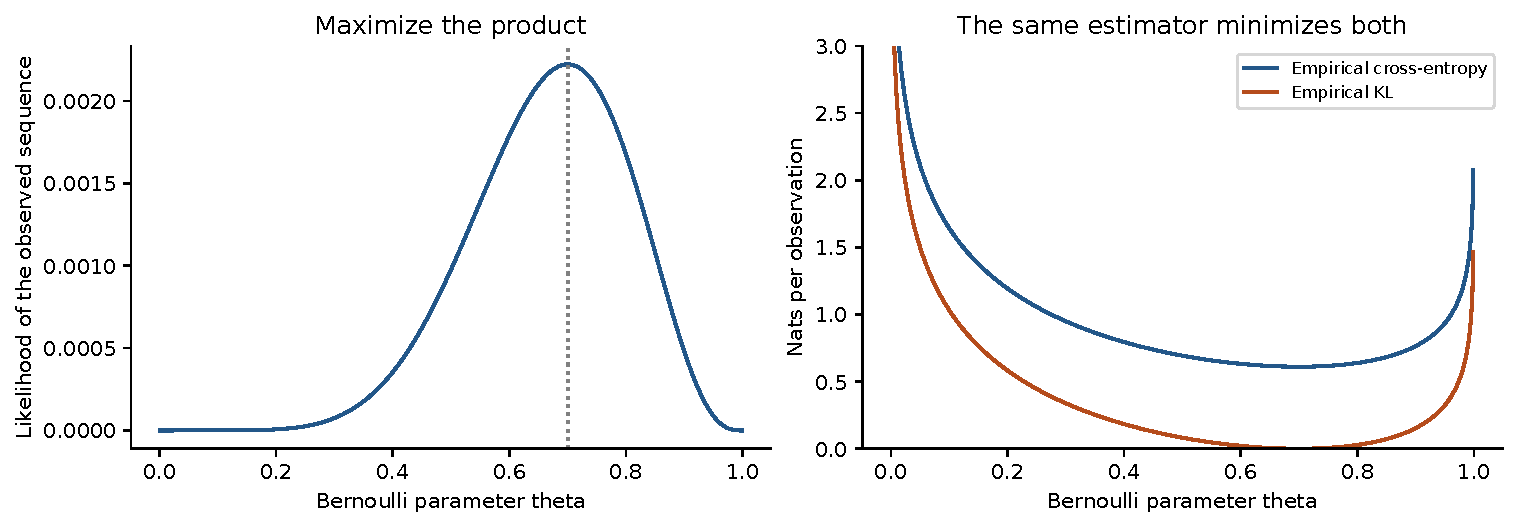
\includegraphics[width=\linewidth]{information_1_2/mle.pdf}
\caption{Seven successes and three failures. The product likelihood peaks at
$0.7$. Mean negative log-likelihood and empirical KL have the same minimizer;
their vertical separation is the entropy of the empirical Bernoulli distribution.}
\end{figure}

For a $K$-class categorical model with counts $n_k$ and probabilities $q_k$,
maximize $\sum_kn_k\log q_k$ subject to $\sum_kq_k=1$.
When all counts are positive, the Lagrangian
\[
\Lambda(q,\lambda)=\sum_kn_k\log q_k+\lambda\left(1-\sum_kq_k\right)
\]
gives $n_k/q_k=\lambda$. Summing $q_k=n_k/\lambda$ gives $\lambda=m$, so
$q_k=n_k/m$. Concavity of the log objective makes this a global optimum.
Zero-count classes obtain zero probability in the unrestricted closed simplex;
this can produce infinite future log loss if a previously unseen class appears.
Pseudocounts or priors can address that issue, but then the estimator is no
longer this unregularized maximum-likelihood estimator. With a finite softmax
parameterization, zero probabilities are approached only as limits.

\subsection{Continuous data: densities are not point probabilities}
A continuous measurement such as position has $P(X=x)=0$ at every individual
point, so a continuous-data likelihood uses a \emph{density} $q_\theta(x)$, not
point mass. For a small measurement bin of width $\Delta$,
\[
P_\theta(x\leq X<x+\Delta)\approx q_\theta(x)\Delta.
\]
With a fixed measurement scale, the product of $\Delta$ factors does not depend
on $\theta$, explaining why maximizing the density likelihood is meaningful.
A density can exceed one, and a negative log density can be negative.

For densities $p,q$ relative to the same base measure, define differential
entropy and cross-entropy when the integrals exist:
\[
h(P)=-\int p(x)\log p(x)\,dx,\qquad
h(P,Q)=-\int p(x)\log q(x)\,dx.
\]
Unlike discrete entropy, differential entropy can be negative and depends on
units. For $U=aX+b$, $a\ne0$, change of variables yields
\[
p_U(u)=\frac{p_X((u-b)/a)}{|a|},\qquad
h(U)=h(X)+\log|a|.
\]
Converting meters to centimeters adds $\log100$ nats. Differential entropy by
itself is therefore not an absolute number of bits needed to encode a real
number exactly. Fine quantization gives, under appropriate regularity,
$H(X_\Delta)\approx h(X)+\log(1/\Delta)$ in one dimension.

By contrast,
\[
D_{\mathrm{KL}}(P\|Q)=\int p(x)\log\frac{p(x)}{q(x)}\,dx
\]
is invariant under a common invertible smooth coordinate transformation: the
Jacobian factors cancel inside the density ratio, and the outer measure changes
consistently. It remains nonnegative, and it equals $h(P,Q)-h(P)$ when that
subtraction is well defined.

\begin{warning}[A subtle limit of the empirical-KL shorthand]
For continuous observations, the empirical measure is
$\hat P_m=m^{-1}\sum_i\delta_{x^{(i)}}$, a collection of point masses.
A smooth density model assigns zero probability to that finite set, whereas
$\hat P_m$ assigns it probability one. Thus
$D_{\mathrm{KL}}(\hat P_m\|Q_\theta)=+\infty$ in the literal measure-theoretic
sense. The finite sample negative log-density is still a valid MLE objective,
but it is not a finite KL between those two measures. Use the population-density
KL interpretation, or explicitly discretize/smooth consistently. The discrete
chain in \eqref{eq:info12-mlechain} should not be transferred blindly to Dirac
empirical measures and continuous densities.
\end{warning}

This issue does not invalidate conditional classification: for each observed
input, the predicted distribution over a finite set of labels is discrete.
The per-example categorical cross-entropy remains well defined even when the
input itself is continuous.

\subsection{Interpreting the slide: approximating two modes by one Gaussian}
Suppose a robot's position belief has two plausible locations because two
corridors look similar. Use the explicit illustrative density
\[
p(x)=\tfrac12\mathcal N(x;-3,0.7^2)+\tfrac12\mathcal N(x;3,0.7^2).
\]
We are forced to summarize it with a single Gaussian
$q_{\mu,s}(x)=\mathcal N(x;\mu,s^2)$, $s>0$. No member of this family can
represent both narrow peaks faithfully. Which compromise does each KL choose?

\paragraph{Forward KL: derive the moment-matching solution.}
Minimizing $D_{\mathrm{KL}}(P\|Q_{\mu,s})$ is equivalent to minimizing
$\mathbb E_P[-\log q_{\mu,s}(X)]$, because $h(P)$ is constant. The Gaussian
negative log density gives
\[
h(P,Q_{\mu,s})=\frac12\log(2\pi s^2)
+\frac{\mathbb E_P[(X-\mu)^2]}{2s^2}.
\]
Let $m_P=\mathbb E_P X$ and $v_P=\operatorname{Var}_P X$. Expanding
$X-\mu=(X-m_P)+(m_P-\mu)$ and noting the cross term has mean zero gives
\[
\mathbb E_P[(X-\mu)^2]=v_P+(m_P-\mu)^2.
\]
For any $s$, the minimizing mean is $\mu=m_P$. Write $v=s^2$; then
\[
\frac{d}{dv}\left[\frac12\log(2\pi v)+\frac{v_P}{2v}\right]
=\frac{v-v_P}{2v^2}.
\]
It is negative below $v_P$ and positive above, so the minimizing variance is
$v=v_P$ when $v_P>0$. For our symmetric mixture,
\[
\boxed{\mu^*=0,\qquad(s^*)^2=3^2+0.7^2=9.49,
\qquad s^*\approx3.0806.}
\]
The broad fitted Gaussian covers both modes, even though it assigns appreciable
density to the low-probability region between them. Ignoring either mode would
make many $P$-drawn observations extremely surprising. That is what forward KL
penalizes. The mean position zero is a statistical summary, not necessarily a
physically plausible robot location.

\paragraph{Reverse KL: why a single mode can win.}
The reverse objective is
\[
D_{\mathrm{KL}}(Q_{\mu,s}\|P)
=\mathbb E_Q[\log q_{\mu,s}(X)-\log p(X)]
=-h(Q_{\mu,s})-\mathbb E_Q\log p(X).
\]
Now the fitted model supplies the samples. A broad $Q$ generates many samples
between the two peaks, where $p(x)$ is tiny, producing a large penalty. A narrow
$Q$ centered near one peak rarely visits the valley or the other peak. Missing
the other mode is less directly penalized because expectations are under $Q$.
The $-h(Q)$ term matters too: it discourages collapsing a continuous Gaussian
to an infinitesimally narrow spike. Reverse KL is not merely ``maximize $p$ at
the model mean.''

Near the left mode, if the peaks are well separated,
$p(x)\approx\tfrac12\mathcal N(x;-3,0.7^2)$. Choosing $Q$ close to that component
makes $\log(q/p)\approx\log2$, so its reverse KL is roughly $0.6931$ nats.
The companion script searches Gaussian mean and scale on a grid, refines the
best grid neighborhood, and evaluates expectations by Gauss--Hermite quadrature.
It finds a fit near $(\mu,s)=(-3,0.7)$ with reverse KL about $0.69312$.
By symmetry a corresponding fit near $(3,0.7)$ has the same value. This numerical
search supports the displayed example; it is not a theorem that reverse KL
always selects exactly one mode or a proof of global optimality for every
mixture.

\begin{figure}[htbp]
\centering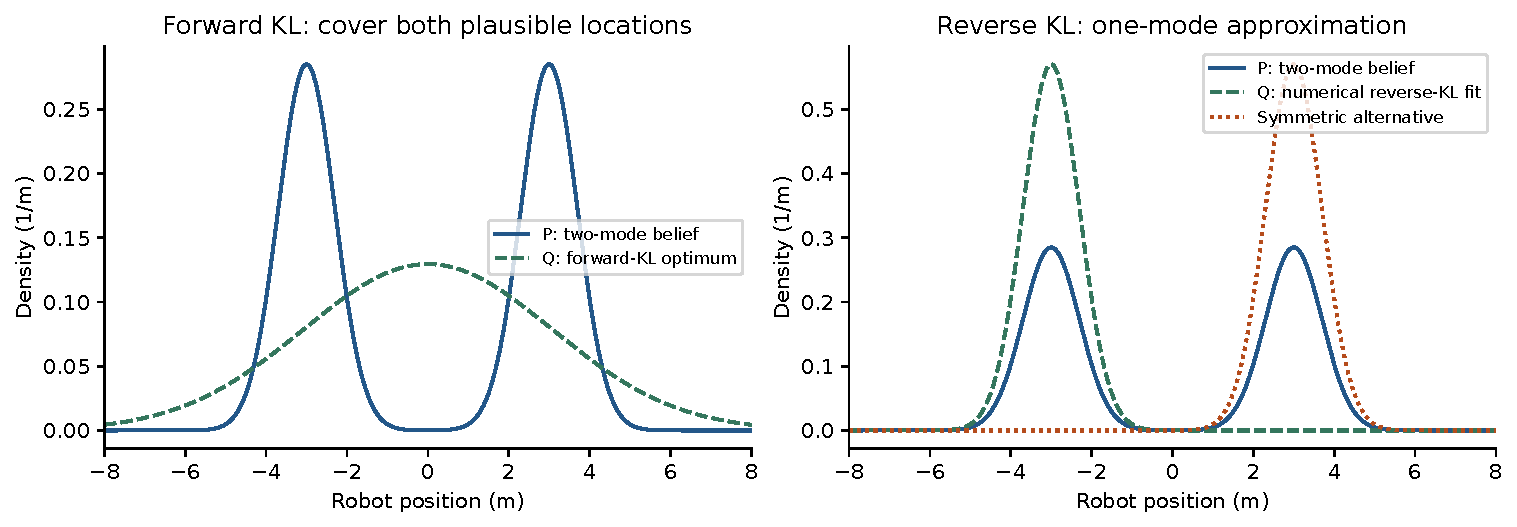
\includegraphics[width=\linewidth]{information_1_2/mixture_direction.pdf}
\caption{A constructed counterpart of the slide's qualitative example, with
explicit distributions. Forward KL has an analytically derived Gaussian optimum.
Reverse KL has two symmetric one-mode candidates found numerically. The mismatch
is unavoidable because a single Gaussian cannot express this two-mode belief.}
\end{figure}

\begin{figure}[htbp]
\centering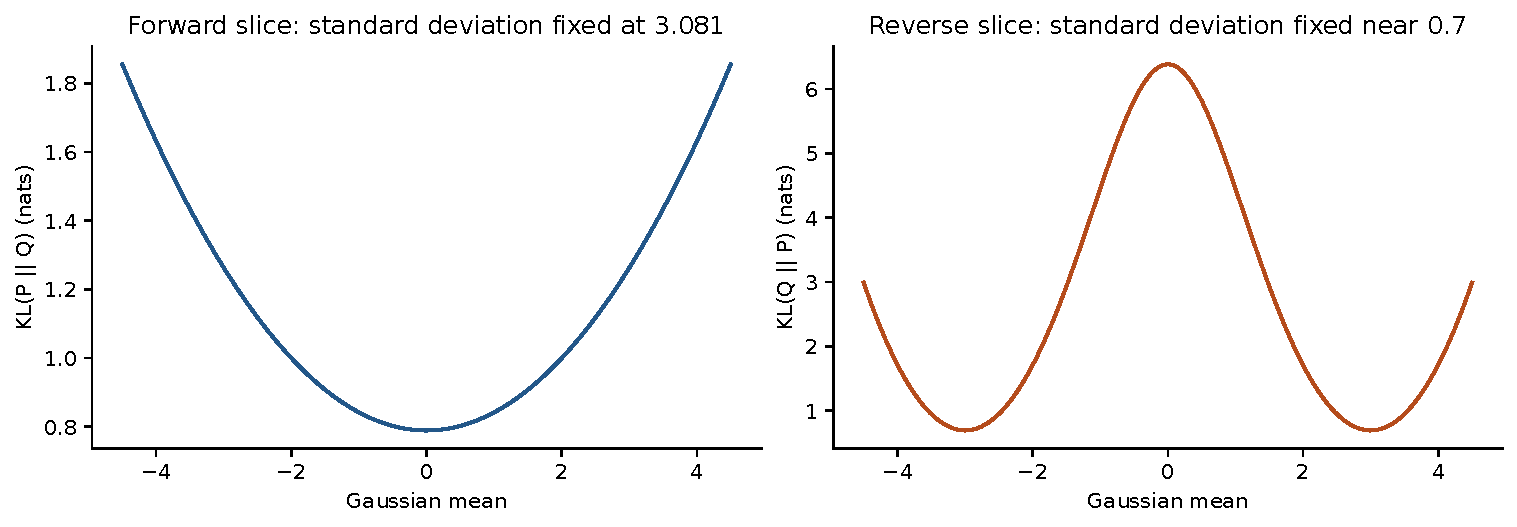
\includegraphics[width=\linewidth]{information_1_2/mixture_objectives.pdf}
\caption{One-dimensional slices through two different objectives. Each panel
holds the standard deviation at its displayed fitted value and varies the mean.
The forward slice favors the midpoint; the reverse slice favors either peak.
These slices are not the full two-parameter optimization landscapes.}
\end{figure}

\paragraph{When the slogan fails.}
``Forward KL covers modes; reverse KL seeks modes'' is a useful tendency for
restricted approximating families and well-separated targets. If the family
contains $P$, both directions can achieve the exact match. Overlapping modes,
unequal mixture weights, or a richer family can change the compromise. Neither
direction is universally better. For localization, throwing away a plausible
mode can hide ambiguity, while a broad Gaussian can place probability in
impossible corridors. A multimodal representation may be preferable to either
single-Gaussian approximation.

\paragraph{Why maximum likelihood is the left-hand case.}
MLE averages $-\log q_\theta(x)$ over \emph{observed data}. It asks whether the
model makes the data plausible, giving forward KL in the population/discrete
interpretation. It does not sample from $Q_\theta$ and ask whether those samples
are plausible under $P$. Reverse-KL objectives arise in other settings, but do
not follow from the likelihood derivation just given.

\subsection{Transfer question 1: why track KL rather than cross-entropy?}
Because KL removes the uncertainty floor. A perfect model of a fair binary
source still has cross-entropy $\log2\approx0.6931$ nats. A perfect model of a
source with probabilities $(0.95,0.05)$ has cross-entropy about $0.1985$ nats.
Both have KL zero. A larger cross-entropy does not necessarily mean the model is
further from its source; the source may simply be less predictable.

For a fixed known $P$, KL states the excess expected loss relative to the
unrestricted optimum $Q=P$. For example, if $H(P)=0.60$ and $H(P,Q)=0.65$,
the model pays $0.05$ extra nats per observation. Cross-entropy alone would not
reveal that gap unless we knew the entropy floor.

\paragraph{Three qualifications make this useful in practice.}
First, with $P$ fixed, subtracting $H(P)$ leaves gradients and optimizer locations
unchanged. Computing KL does not improve optimization by itself. Second, if the
model family cannot represent $P$, its best attainable KL may be positive.
The actual optimization gap within that family is
\[
D_{\mathrm{KL}}(P\|Q_\theta)-\inf_{\vartheta}
D_{\mathrm{KL}}(P\|Q_\vartheta),
\]
not simply $D_{\mathrm{KL}}(P\|Q_\theta)$. Third, true $P$ and its entropy are
usually unknown. Held-out samples let us estimate cross-entropy, while estimating
entropy accurately can be difficult, especially in high dimensions.

If labels are represented by one-hot targets, the target entropy for each
example is zero, so per-example cross-entropy and KL to that point mass are
numerically the same. That does not prove the true conditional label entropy is
zero. With noisy or ambiguous labels, the real uncertainty can remain positive.
Known simulator distributions, repeated outcomes at the same finite context,
or soft target distributions are settings in which the entropy subtraction can
be directly informative.

\subsection{Transfer question 2: derive binary cross-entropy as a special case}
For an input $x_n$, the model's distribution over labels $0,1$ is
\[
Q_n=(1-\hat y_n,\hat y_n),\qquad
\hat y_n=p_w(Y=1\mid x_n).
\]
The observed label $y_n\in\{0,1\}$ defines a target distribution concentrated on
that outcome:
\[
P_n=(1-y_n,y_n).
\]
Substituting these two probability vectors into the general finite-outcome
cross-entropy, with the sum over \emph{labels}, gives
\begin{align*}
H(P_n,Q_n)
&=-\sum_{k\in\{0,1\}}P_n(k)\log Q_n(k)\\
&=-(1-y_n)\log(1-\hat y_n)-y_n\log\hat y_n.
\end{align*}
Averaging over the $N$ observations gives exactly the lecture formula:
\[
\boxed{L(w)=-\frac1N\sum_{n=1}^N
\left[y_n\log\hat y_n+(1-y_n)\log(1-\hat y_n)\right].}
\]
There are two different averages: the inner sum is over possible labels at a
fixed input; the outer sum is over dataset examples. The labels and predictions
across all examples are not themselves one normalized probability vector.

An equivalent joint construction avoids ambiguity: put mass $1/N$ on each
example index $n$, and define
$P(n,k)=N^{-1}\mathbf1\{k=y_n\}$ and
$Q_w(n,k)=N^{-1}Q_n(k)$. Then
\[
H(P)=\log N,\quad H(P,Q_w)=\log N+L(w),\quad
D_{\mathrm{KL}}(P\|Q_w)=L(w).
\]
This index-based joint space is not the same as grouping repeated inputs into
an empirical conditional label distribution, whose entropy may be positive.
Both constructions produce the same averaged conditional log loss; they assign
entropy to different random variables.

\paragraph{Soft targets and more than two classes.}
If a target supplies a probability $r_n\in[0,1]$ rather than a hard label,
replace $y_n$ by $r_n$. The same formula becomes the cross-entropy between two
Bernoulli distributions. Its KL equals that BCE minus the target entropy.
For $K$ classes, target probabilities $r_{nk}$ and predictions $q_{nk}$ give
\[
L=-\frac1N\sum_n\sum_{k=1}^K r_{nk}\log q_{nk}.
\]
With one-hot targets this reduces to the negative log probability of the correct
class. Label smoothing changes the target distribution, hence also its entropy
and the optimum; it is not merely a different algebraic form of the original
hard-label objective.

\subsection{Worked semantic-perception example: separate uncertainty from error}
Consider a robot semantic classifier with labels free space, person, and cart.
For a transparent teaching example, the input has only two discrete contexts:
open floor and occluded view. In 100 observations of each context, the label
counts are
\begin{center}
\begin{tabular}{lrrr}
\toprule
Context & Free & Person & Cart\\
\midrule
Open floor & 80 & 15 & 5\\
Occluded view & 10 & 20 & 70\\
\bottomrule
\end{tabular}
\end{center}
The empirical conditional distributions are
$\hat P_A=(0.80,0.15,0.05)$ and $\hat P_B=(0.10,0.20,0.70)$.
Suppose a model predicts
$Q_A=(0.70,0.20,0.10)$ and $Q_B=(0.20,0.30,0.50)$.
Both contexts have weight $1/2$ in this dataset. Directly from the counts,
\[
\mathrm{NLL}_{\mathrm{mean}}
=-\frac1{200}\sum_{c\in\{A,B\}}\sum_k n_{ck}\log Q_c(k)
\approx0.764413\ \text{nats}.
\]
The empirical conditional entropy and mismatch are
\begin{align*}
\hat H(Y\mid X)&=\tfrac12H(\hat P_A)+\tfrac12H(\hat P_B)
\approx0.707344,\\
\hat D&=\tfrac12D_{\mathrm{KL}}(\hat P_A\|Q_A)
+\tfrac12D_{\mathrm{KL}}(\hat P_B\|Q_B)
\approx0.057069.
\end{align*}
They add to $0.764413$, as predicted by \eqref{eq:info12-conditional}.
An unrestricted categorical model per context would fit the empirical frequencies
and reduce the empirical KL to zero, but its cross-entropy would remain
$0.707344$. The remaining label variation cannot be predicted from these two
context categories in this empirical model.

\begin{figure}[htbp]
\centering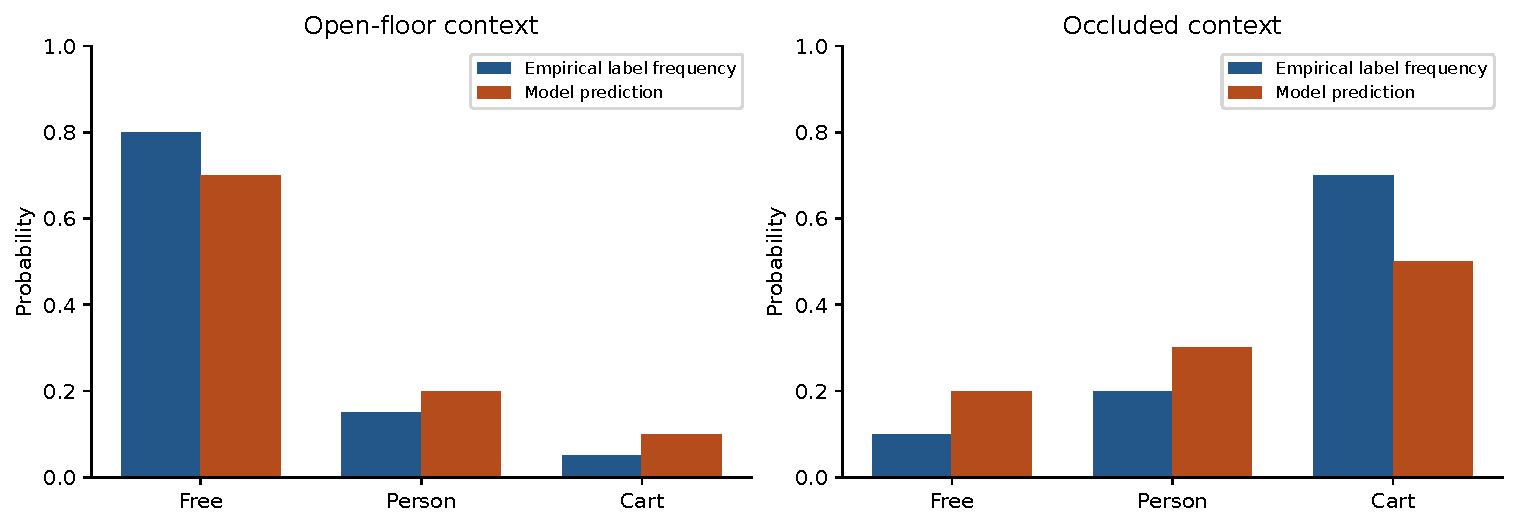
\includegraphics[width=\linewidth]{information_1_2/conditional_robot.pdf}
\caption{The robot example's target frequencies and model probabilities.
The occluded context underpredicts carts; the resulting conditional KL measures
that mismatch separately from the label variability within each context.}
\end{figure}

This is an in-sample decomposition of constructed counts, not an estimate of
irreducible uncertainty on all future robot observations. Richer inputs might
resolve ambiguity; finite frequencies are noisy; context proportions can shift.
For a real study, fit models on training data, compare predictive log loss on
held-out objects or sessions, and report how any entropy estimate was obtained.
Do not estimate an entropy floor from the same overfit model and then call it
known ground truth.

\subsection{Implement the definitions without hiding their edge cases}
The companion uses NumPy for the definitions and numerical experiments.
A stable finite-distribution KL calculation must ignore zero $P$ terms while
returning infinity when positive $P$ meets zero $Q$:
\begin{lstlisting}
def kl(p, q):
    p = np.asarray(p, dtype=float)
    q = np.asarray(q, dtype=float)
    # Validate matching shapes, nonnegativity and sums of one first.
    active = p > 0
    if np.any(q[active] == 0):
        return float("inf")
    return np.sum(p[active] *
                  (np.log(p[active]) - np.log(q[active])))
\end{lstlisting}
The full script validates probability vectors and supports bits or nats.
Using a mask before evaluating logarithms avoids invalid inactive terms.
Adding an arbitrary epsilon to every probability changes the distributions and
may destroy normalization. If smoothing is intended, define and normalize the
smoothed model explicitly. For network outputs, compute log probabilities from
logits using stable log-sum-exp; avoid taking logs after probabilities have
rounded to zero.

In the mixture example, use
\[
\log p(x)=\operatorname{logaddexp}
\bigl(\log\mathcal N(x;-3,0.7^2),
      \log\mathcal N(x;3,0.7^2)\bigr)-\log2.
\]
Computing each tiny density and adding them first can underflow in the tails.
For reverse KL, write $X=\mu+sZ$, $Z\sim\mathcal N(0,1)$, and integrate over
$Z$. Gauss--Hermite quadrature approximates this expectation without truncating
the real line to a plotting window. The script checks the selected candidate
with both 120 and 240 quadrature nodes; their reverse-KL estimates differ by
less than $10^{-8}$ for this example. Numerical integration and grid search
remain approximations, not symbolic proofs of an optimum.

\paragraph{Reproduce and inspect.}
From the repository root:
\begin{lstlisting}[language=bash]
python deep_learning/code/information_1_2.py
make dl
\end{lstlisting}
Seven vector figures and a numerical summary are written under
\path{deep_learning/figures/information_1_2/}. Committed figures allow the notes
to compile without running Python. The script checks the entropy decomposition,
KL support cases, empirical-NLL equivalence, the BCE special case, and coordinate
invariance for a Gaussian KL. It uses no machine-learning library and labels all
examples as constructed data.

\subsection{Reasoning exercises}
Try these before the worked answers. Explain what distribution supplies the
expectation in every expression, rather than starting with algebra alone.
\begin{exercise}[An exact code]
For $P=(1/2,1/4,1/8,1/8)$, use the three codebooks above to verify each expected
length. How many extra ideal bits does the uniform code use over 1,000 i.i.d.
events on average? Does this say every sequence uses exactly that many extra bits?
\end{exercise}
\begin{exercise}[Asymmetry and impossible events]
Evaluate both KL directions for $P=(1,0)$ and $Q=(1/2,1/2)$ in bits.
Which expectation encounters an impossible event, and under which model?
\end{exercise}
\begin{exercise}[MLE without a remembered formula]
For a categorical dataset with counts $(12,6,2)$, derive its unrestricted MLE
using a Lagrange multiplier. What changes if the last count is zero?
\end{exercise}
\begin{exercise}[Two sources, the same reported loss]
Two models each have cross-entropy $0.7$ nats. Their source entropies are $0.69$
and $0.2$. Which model is closer in forward KL to its own source? Can you infer
which has higher classification accuracy?
\end{exercise}
\begin{exercise}[Moments and modes]
For $P=\tfrac12\mathcal N(-a,s_0^2)+\tfrac12\mathcal N(a,s_0^2)$, derive the
forward-KL Gaussian mean and variance. Explain what happens as $a\to0$ and why
this limits a universal ``reverse KL chooses one peak'' slogan.
\end{exercise}
\begin{exercise}[One-hot targets are not a population claim]
A repeated input produces label one in $70\%$ of trials. What probability
minimizes expected BCE? Why can every observed one-hot target have zero entropy
while the conditional source entropy is positive?
\end{exercise}

\subsection{Worked answers and checks on interpretation}
\paragraph{1. Coding.}
The averages are $1.75$, $2$, and $2.625$ bits per event. The uniform code costs
$0.25\times1000=250$ extra bits in expectation. Individual sequences have
fluctuating outcome counts, so the realized difference need not equal 250.
The statement concerns an average under the source distribution.

\paragraph{2. Support.}
$D_{\mathrm{KL}}(P\|Q)=\log_2(1/(1/2))=1$ bit. The reverse direction is infinite:
$Q$ samples the second event with probability $1/2$, but $P$ assigns it zero
probability. In the forward direction that event is never sampled.

\paragraph{3. Categorical MLE.}
The stationary equations give $q_k=n_k/\lambda$ and $\lambda=20$, hence
$(0.6,0.3,0.1)$. If the dataset instead has counts $(12,6,0)$, its total is 18
and the closed-simplex optimum is $(2/3,1/3,0)$. A finite softmax can approach but
not reach this boundary. A future third-class observation would have infinite
loss under the unsmoothed boundary solution.

\paragraph{4. Excess loss.}
The KL values are $0.01$ and $0.5$ nats. The first is much closer in this directed
log-loss sense, even though raw cross-entropies agree. Classification accuracy
cannot be inferred from these quantities alone: it discards confidence and also
depends on a decision rule and the source distribution.

\paragraph{5. Gaussian approximation.}
The mean is zero by symmetry. The second moment is $a^2+s_0^2$, so the variance
is also $a^2+s_0^2$. As $a\to0$, the mixture becomes one Gaussian and both KL
directions can achieve zero with that same Gaussian. The two-mode behavior is
about approximating a separated multimodal target with a restricted family.

\paragraph{6. Label noise.}
The expected loss is $-0.7\log p-0.3\log(1-p)$ and is minimized at $p=0.7$.
Each realized label defines a point mass with entropy zero, but before the
outcome is known the conditional label distribution is Bernoulli$(0.7)$, with
entropy about $0.610864$ nats. An observed target and the process generating
successive targets are different distributions.

\begin{keyidea}[A way to reconstruct the whole section]
Read the expectation first: it tells you who supplies the outcomes. Then read
the logarithm: it tells you whose probabilities judge them. If both are $P$,
you measure entropy. If $P$ supplies outcomes and $Q$ scores them, you measure
cross-entropy. Their excess is forward KL. Replacing the unknown source
expectation by an empirical average gives the negative log-likelihood used for
learning. Always identify the outcome space, conditioning, support, and log unit
before manipulating the formula.
\end{keyidea}

\paragraph{Relation to the lecture and further reading.}
This section expands the supplied entropy, KL, and maximum-likelihood slides,
including both transfer questions and the qualitative two-mode diagram. The
new diagrams use explicitly specified distributions and reproducible calculations.
For the lecture's textbook context, see \citet{goodfellow2016deep}, Chapter 3,
Section 3.13 and Figure 3.6, and Chapter 5, Section 5.5 (especially the
maximum-likelihood equivalences). The finite-code qualifications and the
continuous empirical-measure distinction above specify the assumptions needed
to interpret the concise slide statements carefully.

% ============================================================
%  1.3 Logistic Regression as a Neural Network: The Perceptron
% ============================================================
\section{Logistic Regression as a Neural Network: The Perceptron}
\label{sec:logreg_to_mlp:logistic_regression_as_a_neural_network_the_perceptron}

% Notes go here.

% Section 1.4: from fixed features to learned representations.
\section{Multilayer Perceptrons}
\label{sec:logreg_to_mlp:multilayer_perceptrons}

\subsection{Why add a hidden layer?}
A sigmoid neuron can turn an affine score into a probability, but its $1/2$ decision boundary is still a hyperplane in its input features. If the relationship between those features and the label cannot be separated by a hyperplane, adjusting the sigmoid neuron alone cannot solve the representation problem.

Consider two binary measurements $x_1,x_2$ and a label indicating that exactly one measurement is active:
\[
 (0,0)\mapsto0,\qquad(1,0)\mapsto1,\qquad
 (0,1)\mapsto1,\qquad(1,1)\mapsto0.
\]
This is XOR. To classify it with $\hat y=\mathbf{1}\{w_1x_1+w_2x_2+b\geq0\}$ would require
\[
 b<0,\quad w_1+b\geq0,\quad w_2+b\geq0,\quad w_1+w_2+b<0.
\]
The middle inequalities imply $w_1+w_2+2b\geq0$, hence
$w_1+w_2+b\geq-b>0$, contradicting the last inequality. This is a limitation of the model family, not a failure of an optimizer.

One response is to invent a nonlinear feature, such as $x_1x_2$. Another is to let the model learn features. An MLP does this by composing affine maps and nonlinear activations. Its final sigmoid neuron is logistic regression on the last hidden representation rather than on the raw measurements.
\begin{keyidea}[A hidden layer changes the coordinates used for prediction]
A hidden layer computes $\mathbf{h}(\mathbf{x};\theta)$, a collection of parameterized features. The output model combines those features. Joint learning adjusts both how the input is represented and how the representation is used. A hidden unit is called hidden because it is an internal computation, not an observed target variable.
\end{keyidea}

\subsection{Derive a layer from its individual neurons}
We follow the lecture convention here: inputs are columns, and each neuron's incoming weight vector is a column of $W$. For $k_1$ neurons,
\[
 W^{(1)}=[\mathbf{w}^{(1)}_1\ \cdots\ \mathbf{w}^{(1)}_{k_1}]
 \in\mathbb{R}^{d\times k_1},\qquad
 \mathbf{b}^{(1)}\in\mathbb{R}^{k_1}.
\]
Neuron $j$ computes
\[
 z^{(1)}_j=\sum_{i=1}^d W^{(1)}_{ij}x_i+b^{(1)}_j,
 \qquad h^{(1)}_j=g^{(1)}(z^{(1)}_j).
\]
Stacking these $k_1$ equations gives
\begin{align}
 \underbrace{\mathbf{z}^{(1)}}_{k_1\times1}
 &=\underbrace{W^{(1)\mathsf T}}_{k_1\times d}
   \underbrace{\mathbf{x}}_{d\times1}
   +\underbrace{\mathbf{b}^{(1)}}_{k_1\times1},\\
 \underbrace{\mathbf{h}^{(1)}}_{k_1\times1}
 &=g^{(1)}\!\left(\underbrace{\mathbf{z}^{(1)}}_{k_1\times1}\right).
\end{align}
The activation is applied elementwise and preserves shape. The weights and bias are learned parameters; $\mathbf{z}^{(1)}$ and $\mathbf{h}^{(1)}$ depend on the current example. All neurons in this layer read the same input vector. They do not receive separate examples.

A fully connected layer connects every input coordinate to every output neuron. Consequently it has $dk_1$ weights and $k_1$ biases. The number of connections counts weights, not independent input data points.

\subsection{Compose two hidden layers and an output layer}
Let the output have $c$ coordinates. Set $\mathbf{h}^{(0)}=\mathbf{x}$. Then
\begin{align}
 \mathbf{z}^{(1)}&=W^{(1)\mathsf T}\mathbf{x}+\mathbf{b}^{(1)},
 &\mathbf{h}^{(1)}&=g^{(1)}(\mathbf{z}^{(1)}),\\
 \mathbf{z}^{(2)}&=W^{(2)\mathsf T}\mathbf{h}^{(1)}+\mathbf{b}^{(2)},
 &\mathbf{h}^{(2)}&=g^{(2)}(\mathbf{z}^{(2)}),\\
 \mathbf{z}^{(3)}&=W^{(3)\mathsf T}\mathbf{h}^{(2)}+\mathbf{b}^{(3)},
 &\hat{\mathbf{y}}&=g^{(3)}(\mathbf{z}^{(3)}).
\end{align}
Here $W^{(2)}\in\mathbb{R}^{k_1\times k_2}$ and
$W^{(3)}\in\mathbb{R}^{k_2\times c}$. The output activation depends on the task: a sigmoid for one binary probability, softmax for mutually exclusive classes, or often the identity for unconstrained regression. Hidden activations need not match the output activation.

\begin{figure}[htbp]
\centering
\begin{tikzpicture}[>=Stealth, every node/.style={font=\small},node distance=0.65cm]
\node[draw,rounded corners,align=center] (x) {Input\\$d$ coordinates};
\node[draw,rounded corners,align=center,right=of x] (h1) {Hidden 1\\$k_1$ features};
\node[draw,rounded corners,align=center,right=of h1] (h2) {Hidden 2\\$k_2$ features};
\node[draw,rounded corners,align=center,right=of h2] (y) {Output\\$c$ coordinates};
\draw[->] (x)--(h1); \draw[->] (h1)--(h2); \draw[->] (h2)--(y);
\node[below=0.5cm of h1] {$dk_1$ weights};
\node[below=0.5cm of h2] {$k_1k_2$ weights};
\node[below=0.5cm of y] {$k_2c$ weights};
\end{tikzpicture}
\caption{A forward pass has three affine maps when there are two hidden layers and an output layer. The input is not counted as a computed layer. Each arrow denotes a full matrix transformation followed by an activation.}
\end{figure}

For one hidden layer, the nested form is
\[
 \hat{\mathbf{y}}=g^{(2)}\!\left(W^{(2)\mathsf T}
 g^{(1)}(W^{(1)\mathsf T}\mathbf{x}+\mathbf{b}^{(1)})+\mathbf{b}^{(2)}\right).
\]
The nesting records a dependency: the second layer must wait for the first layer's features. Neurons within a layer can be evaluated together, while successive layers depend on earlier results. A network with only affine maps and elementwise activations also processes different batch examples independently.

\subsection{Why the hidden nonlinearity matters: a proof}
Suppose two consecutive layers have identity activations. Write their affine maps as $A_1\mathbf{x}+\mathbf{b}_1$ and $A_2\mathbf{h}+\mathbf{b}_2$. Substitution gives
\[
 A_2(A_1\mathbf{x}+\mathbf{b}_1)+\mathbf{b}_2
 =\underbrace{A_2A_1}_{A_{\mathrm{eff}}}\mathbf{x}
  +\underbrace{(A_2\mathbf{b}_1+\mathbf{b}_2)}_{\mathbf{b}_{\mathrm{eff}}}.
\]
Induction collapses any finite stack of affine maps into a single affine map. Adding only linear hidden layers therefore cannot solve XOR; with a final sigmoid it is still logistic regression on an affine score. Factorization can affect optimization or impose a rank constraint, but does not produce nonlinear decision geometry.

With $g(z)=\max(0,z)$ (ReLU), each unit can turn off on one side of its own hyperplane. Different inputs activate different subsets of units. Within a fixed activation pattern the map is affine; across patterns it is piecewise affine. This permits several boundary pieces in input space. ReLU is differentiable except at zero, so the slides' differentiability requirement should be read with this common almost-everywhere qualification; learning implementations choose a derivative convention at the kink.

\subsection{A constructive nonlinear representation: solve XOR by hand}
Choose two ReLU features
\[
 h_1=\max(0,x_1-x_2),\qquad
 h_2=\max(0,x_2-x_1).
\]
Their sum is $|x_1-x_2|$. At the four binary inputs:
\begin{center}
\begin{tabular}{ccccc}
\toprule
$(x_1,x_2)$ & $h_1$ & $h_2$ & $h_1+h_2$ & $y$\\
\midrule
$(0,0)$ & 0 & 0 & 0 & 0\\
$(1,0)$ & 1 & 0 & 1 & 1\\
$(0,1)$ & 0 & 1 & 1 & 1\\
$(1,1)$ & 0 & 0 & 0 & 0\\
\bottomrule
\end{tabular}
\end{center}
Now a single output neuron suffices:
\[
 z_{\mathrm{out}}=10(h_1+h_2-0.5),\qquad
 p=\sigma(z_{\mathrm{out}}).
\]
The negative examples have $p=\sigma(-5)\approx0.0067$, and the positive examples have $p=\sigma(5)\approx0.9933$. In hidden space the boundary is the line $h_1+h_2=0.5$. Its preimage in input space is $|x_1-x_2|=0.5$, comprising two parallel lines. The output remains linear in hidden features even though the boundary is not a single line in the original inputs.

\begin{figure}[htbp]
\centering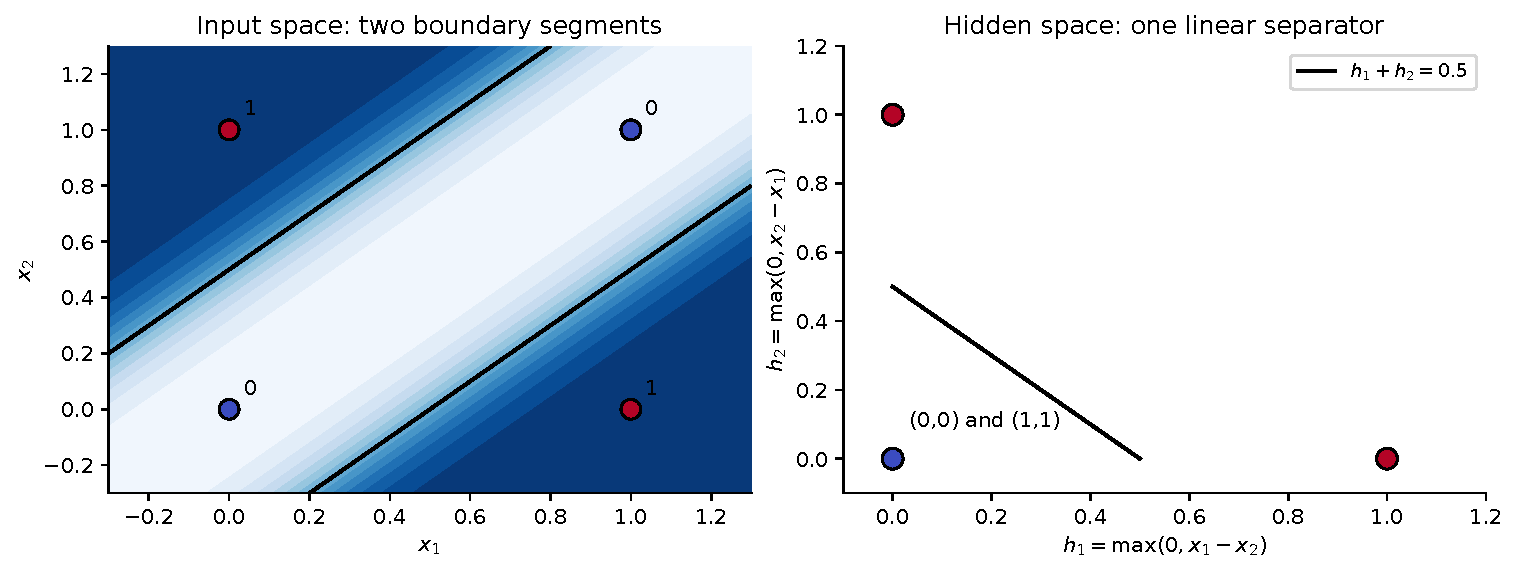
\includegraphics[width=\linewidth]{mlp_1_4_1_5/xor_features.pdf}
\caption{An explicit feature map makes XOR linearly separable. Colors on the left background show the output probability; labeled points are the four binary cases. Both negative examples map to the same hidden point. These features and weights are constructed by hand, demonstrating representability rather than proving a training algorithm will find them.}
\end{figure}

This toy problem has a useful interpretation for perception: two sensors may disagree in a way that predicts a fault, even when either sensor reading alone is uninformative. The learned feature needs to detect a relationship between inputs. Real sensor errors are not literally noiseless XOR, but the example isolates the need for interactions.

Calling hidden units ``adaptable basis functions'' emphasizes this feature-building role. For a scalar output logit,
\[
 z_{\mathrm{out}}=\beta_0+\sum_j\beta_j\phi_j(\mathbf{x};\theta),
\]
where $\phi_j$ are hidden activations. Unlike fixed polynomial features, their parameters can be learned. They need not form a basis in the strict linear-algebra sense: they may be redundant, dependent, or inactive. Also, learning the hidden parameters jointly generally removes logistic regression's convexity guarantee.

\subsection{Time complexity for the lecture's two-hidden-layer question}
Assume dense matrices, ordinary matrix multiplication, fixed-precision scalar arithmetic, and elementwise activations with constant work per coordinate. Standard softmax also takes linear work in its number of output coordinates. Keep $c$ explicit because the question does not specify output width.

For one example, layer 1 multiplies a $k_1\times d$ matrix by a $d\times1$ vector. The hint gives $O(k_1d\cdot1)$. Equivalently, $k_1$ neurons each compute a dot product with $d$ terms. Apply the same argument at the next layers:
\begin{center}
\begin{tabular}{llll}
\toprule
Layer & Matrix product & Product cost & Bias/activation cost\\
\midrule
First hidden & $(k_1\times d)(d\times1)$ & $O(dk_1)$ & $O(k_1)$\\
Second hidden & $(k_2\times k_1)(k_1\times1)$ & $O(k_1k_2)$ & $O(k_2)$\\
Output & $(c\times k_2)(k_2\times1)$ & $O(k_2c)$ & $O(c)$\\
\bottomrule
\end{tabular}
\end{center}
Add sequential work; do not multiply the layer costs together:
\[
 T=O(dk_1+k_1k_2+k_2c+k_1+k_2+c)
   =\boxed{O(dk_1+k_1k_2+k_2c)}.
\]
The last simplification assumes positive integer widths. For a scalar binary output ($c=1$), a useful explicit answer is
\[
 \boxed{T=O(dk_1+k_1k_2+k_2)=O(dk_1+k_1k_2).}
\]
If the intended forward pass stops at the second hidden representation, omit the output-layer term. Writing the architecture next to the answer prevents ambiguity. These counts describe arithmetic work, not exact GPU latency or a promise of ideal parallel speedup.

\subsection{Memory complexity: count what must exist}
Time counts operations; memory counts stored numbers. A multiplication can perform many operations without storing every intermediate scalar product. In the lecture hint, $(n\times m)(m\times k)$ stores two operands and a result, giving $O(nm+mk+nk)$, not $O(nmk)$ storage.

Keep all network parameters resident. The exact number of parameters is
\[
 P=\underbrace{dk_1+k_1k_2+k_2c}_{\text{weights}}
  +\underbrace{k_1+k_2+c}_{\text{biases}}.
\]
The input has $d$ numbers. If all preactivations and activations are retained separately, they use $2(k_1+k_2+c)$ numbers, including the final output. Thus one explicit storage model is
\[
 S_{\mathrm{cache}}=P+d+2(k_1+k_2+c).
\]
An implementation may alias some buffers or save only what a particular activation needs, changing constants. The inclusive big-O answer is
\[
 \boxed{S=O(dk_1+k_1k_2+k_2c+d+k_1+k_2+c).}
\]
For $c=1$ this becomes
\[
 \boxed{S=O(dk_1+k_1k_2+d+k_1+k_2)}.
\]
For positive widths, the product terms dominate these vector terms, so $O(dk_1+k_1k_2)$ is also valid. Showing the unsimplified expression demonstrates that input, output, biases, and intermediate vectors were included as requested.

\begin{warning}[Do not call activation memory the total memory]
$O(d+k_1+k_2+c)$ accounts for input and activations only. It omits the matrices needed to execute the forward pass. Conversely, parameters are stored once, not once per example or once every time they are used. Gradients and optimizer state are separate training allocations and are not required for a forward-only inference calculation.
\end{warning}

For inference, once layer 2 has consumed $\mathbf{h}^{(1)}$, that activation can be released if no later operation needs it. With only two hidden layers, caching versus buffer reuse does not change the order of the vector terms. With variable depth and large batches, the distinction becomes significant; Section~\ref{sec:logreg_to_mlp:matrix_dimensions} makes it explicit.

\subsection{A practical sizing example}
Suppose a grasp-success predictor takes 12 measured features, such as geometric clearance, contact estimates, and pose uncertainty summaries. Choose the illustrative architecture
\[
 12\longrightarrow32\longrightarrow16\longrightarrow1.
\]
It uses $12(32)+32(16)+16(1)=912$ weight multiplications per example, plus the corresponding additions and activations. It has $32+16+1=49$ biases, hence $P=961$ parameters. Retaining input and all $Z/H$ vectors uses
\[
 961+12+2(32+16+1)=1071
\]
scalars. At four bytes per scalar this model accounts for 4,284 bytes. This is an array-element count, not actual process memory: array objects, kernel workspace, allocator overhead, and library code are excluded.

For 256 candidate grasps evaluated together, there are $256(912)=233{,}472$ weight products, while there are still only 961 parameters. The network is reused across candidates. Its predictions would require training and validation before being meaningful; the example here is for architecture and resource accounting.

\subsection{Exercises and worked reasoning}
\paragraph{1. Why does depth without nonlinearity not solve XOR?}
Compose the affine maps including their biases. The result is one affine map, whose threshold is a single hyperplane; the four XOR inequalities remain contradictory. A final sigmoid changes probabilities but not that limitation.

\paragraph{2. What if both hidden widths are doubled?}
For fixed $d,c$, the first-layer products double, the hidden-to-hidden products quadruple, and the output-layer products double. The total factor depends on which term dominates. It is not always exactly four.

\paragraph{3. Is one hidden neuron enough for XOR with ReLU and a sigmoid output?}
No. Its logit is $a\max(0,\mathbf{w}^{\mathsf T}\mathbf{x}+b)+c$, a monotone function of the one affine score (possibly decreasing if $a<0$). Thresholding it gives a half-space, all inputs, or no inputs, with possible boundary ties. XOR requires more than one such half-space decision. The two-unit construction above shows sufficiency.

\paragraph{4. Can a large activation value be interpreted as a probability?}
Not in general. ReLU activations can exceed one, can be rescaled with compensating downstream weights, and need not represent a named semantic concept. The probabilistic interpretation comes from the chosen output distribution and loss, not merely from being a neuron.

% Section 1.5: derive arrays from indexed computations before counting costs.
\section{Matrix Dimensions}
\label{sec:logreg_to_mlp:matrix_dimensions}

\subsection{A matrix is an organized collection of scalar equations}
Dimension checking is a way to keep track of meaning: which index identifies an example, which identifies a feature, and which identifies an output neuron? Rather than remembering a transpose by appearance, derive the expression from one output coordinate.

Let $d$ be the input width and $q$ the number of neurons. In the lecture convention, neuron $j$ has a column weight vector $\mathbf{w}_j\in\mathbb{R}^{d\times1}$. Its score is
\[
 z_j=\mathbf{w}_j^{\mathsf T}\mathbf{x}+b_j
     =\sum_{i=1}^d w_{ij}x_i+b_j.
\]
Here $i$ is summed out: it indexes the features contributing to one neuron. The index $j$ survives: it identifies the resulting score. To compute all scores, collect weight vectors into columns,
\[
 W_s=[\mathbf{w}_1\ \cdots\ \mathbf{w}_q]\in\mathbb{R}^{d\times q}.
\]
Then
\[
 \underbrace{\mathbf{z}}_{q\times1}
 =\underbrace{W_s^{\mathsf T}}_{q\times d}
  \underbrace{\mathbf{x}}_{d\times1}
  +\underbrace{\mathbf{b}}_{q\times1},\qquad
 \underbrace{\mathbf{h}}_{q\times1}=g(\underbrace{\mathbf{z}}_{q\times1}).
\]
The subscript $s$ marks the slides' weight storage, to keep it distinct from code notation below. Matrix multiplication performs all the dot products at once; it does not define a different operation from the scalar equations.

\subsection{Batching in the column-vector convention}
Place $B$ examples in columns:
\[
 X_c=[\mathbf{x}^{(1)}\ \cdots\ \mathbf{x}^{(B)}]
 \in\mathbb{R}^{d\times B}.
\]
The batch preactivation matrix has one neuron per row and one example per column:
\begin{equation}
 \underbrace{Z_c}_{q\times B}
 =\underbrace{W_s^{\mathsf T}}_{q\times d}
  \underbrace{X_c}_{d\times B}
  +\underbrace{\mathbf{b}\mathbf{1}_B^{\mathsf T}}_{q\times B},
 \qquad H_c=g(Z_c)\in\mathbb{R}^{q\times B}.
\end{equation}
Entry $(j,n)$ is
\[
 (Z_c)_{jn}=\sum_i(W_s)_{ij}(X_c)_{in}+b_j.
\]
The same $b_j$ is added for every example $n$. Formally, a $q\times1$ matrix cannot be added to a $q\times B$ matrix by ordinary matrix addition. The slides' shorthand ``$+\mathbf{b}$'' means broadcasting, made explicit here by $\mathbf{b}\mathbf{1}_B^{\mathsf T}$. The repeated columns are not different trainable biases.

\subsection{Transpose the whole equation to get row batches}
Code often places examples in rows. Define
\[
 X_r=X_c^{\mathsf T}\in\mathbb{R}^{B\times d},\qquad
 Z_r=Z_c^{\mathsf T}\in\mathbb{R}^{B\times q}.
\]
Using $(AB)^{\mathsf T}=B^{\mathsf T}A^{\mathsf T}$ gives
\begin{align}
 Z_r
 &=\left(W_s^{\mathsf T}X_c+\mathbf{b}\mathbf{1}_B^{\mathsf T}\right)^{\mathsf T}\\
 &=X_c^{\mathsf T}W_s+\mathbf{1}_B\mathbf{b}^{\mathsf T}\\
 &=X_rW_s+\mathbf{1}_B\mathbf{b}^{\mathsf T}.
\end{align}
Since an elementwise activation commutes with transposition,
$H_r=g(Z_r)=H_c^{\mathsf T}$. Nothing about the model has changed.

PyTorch's dense-layer parameter storage uses one neuron's weights per row. Write that matrix as
\[
 W_p=W_s^{\mathsf T}\in\mathbb{R}^{q\times d}.
\]
Consequently, the familiar code expression is
\begin{equation}
 \boxed{\underbrace{Z_r}_{B\times q}
 =\underbrace{X_r}_{B\times d}
  \underbrace{W_p^{\mathsf T}}_{d\times q}
  +\underbrace{\mathbf{1}_B\mathbf{b}^{\mathsf T}}_{B\times q}.}
\end{equation}
This is the formula $Z=XW^{\mathsf T}+B_{\mathrm{bias}}$ in the lecture's coding notation. We use $B_{\mathrm{bias}}$ for the expanded bias matrix so that $B$ alone can denote batch size.

\begin{center}
\begin{tabular}{lll}
\toprule
Object & Lecture columns & PyTorch-style rows\\
\midrule
Batch input & $X_c:d\times B$ & $X_r:B\times d$\\
Stored weights & $W_s:d\times q$ & $W_p:q\times d$\\
Bias as a mathematical column & $\mathbf{b}:q\times1$ & $\mathbf{b}:q\times1$\\
Preactivations & $Z_c:q\times B$ & $Z_r:B\times q$\\
Affine computation & $W_s^{\mathsf T}X_c+\mathbf{b}\mathbf1_B^{\mathsf T}$ & $X_rW_p^{\mathsf T}+\mathbf1_B\mathbf{b}^{\mathsf T}$\\
\bottomrule
\end{tabular}
\end{center}
In NumPy and PyTorch, the bias is typically a one-dimensional array of shape \texttt{(q,)}. It broadcasts over batch rows. A one-dimensional array has no separate row or column orientation; explicitly reshape it when doing column-batch arithmetic.

\begin{warning}[Two independent layout choices]
Changing examples from columns to rows does not logically force a particular weight layout. One could use row batches with $W_s\in\mathbb{R}^{d\times q}$ and write $X_rW_s$, or with $W_p\in\mathbb{R}^{q\times d}$ and write $X_rW_p^{\mathsf T}$. Both are correct. The letters alone do not specify the convention: the index meanings and dimensions do. PyTorch is not a different mathematics.
\end{warning}
The official \href{https://docs.pytorch.org/docs/stable/generated/torch.nn.Linear.html}{\texttt{torch.nn.Linear} documentation} stores weights with output features in rows and input features in columns, using transformation $xA^{\mathsf T}+b$. It also permits leading dimensions beyond a single batch dimension: the last dimension is the feature dimension. Thus ``PyTorch inputs are row vectors'' is a useful two-dimensional batch convention, not a restriction on every supported tensor.

\subsection{Work through every entry of a concrete batch}
Take two examples, three input features, and two neurons:
\[
 X_r=\begin{bmatrix}1&2&3\\-1&0&2\end{bmatrix},\quad
 W_p=\begin{bmatrix}1&-1&2\\0&3&-1\end{bmatrix},\quad
 \mathbf{b}=\begin{bmatrix}0.5\\-0.5\end{bmatrix}.
\]
The product and broadcast bias are
\[
 X_rW_p^{\mathsf T}=\begin{bmatrix}5&3\\3&-2\end{bmatrix},\qquad
 \mathbf1_2\mathbf{b}^{\mathsf T}=\begin{bmatrix}0.5&-0.5\\0.5&-0.5\end{bmatrix}.
\]
For example, the first example's second neuron gives
$1(0)+2(3)+3(-1)-0.5=2.5$. Every other cell follows the same rule:
\[
 Z_r=\begin{bmatrix}5.5&2.5\\3.5&-2.5\end{bmatrix},\qquad
 H_r=\operatorname{ReLU}(Z_r)=\begin{bmatrix}5.5&2.5\\3.5&0\end{bmatrix}.
\]
Row 2 always belongs to example 2; column 2 always belongs to neuron 2. This semantic identity is as important as whether an array multiplication happens to run.

\begin{figure}[htbp]
\centering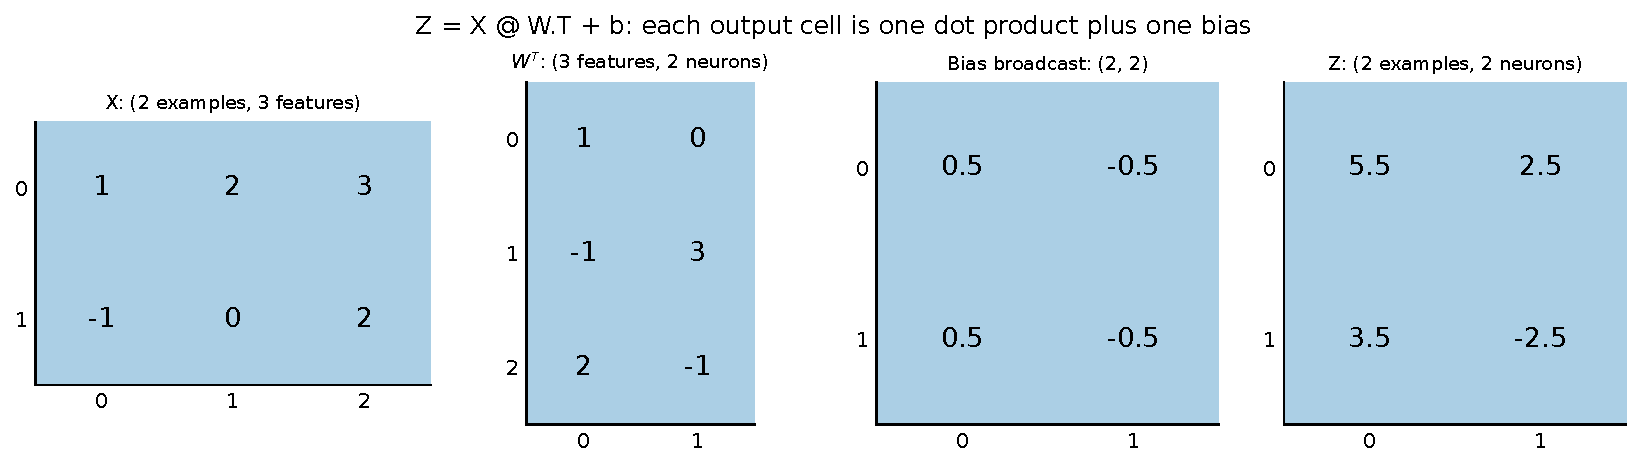
\includegraphics[width=\linewidth]{mlp_1_4_1_5/matrix_example.pdf}
\caption{The batch computation with actual numbers. Output entry $(n,j)$ combines row $n$ of $X$ with column $j$ of $W^{\mathsf T}$, then adds bias $b_j$.}
\end{figure}

\subsection{The lecture's batched-perceptron repetition question}
For one sigmoid output neuron and $B$ examples of dimension $d$, the two requested formulas in row-batch notation are
\begin{align}
 \underbrace{Z}_{B\times1}
 &=\underbrace{X}_{B\times d}
   \underbrace{W^{\mathsf T}}_{d\times1}
   +\underbrace{\mathbf1_B}_{B\times1}\underbrace{b}_{\text{scalar}},
 \qquad W\in\mathbb{R}^{1\times d},\\
 \underbrace{H}_{B\times1}&=\sigma(\underbrace{Z}_{B\times1}).
\end{align}
Equivalently, with examples in columns,
\[
 \underbrace{Z_c}_{1\times B}
 =\underbrace{\mathbf{w}^{\mathsf T}}_{1\times d}
  \underbrace{X_c}_{d\times B}+\underbrace{b\mathbf1_B^{\mathsf T}}_{1\times B},
 \qquad H_c=\sigma(Z_c)\in\mathbb{R}^{1\times B}.
\]
The $B$ probabilities are predictions for different examples, not probabilities of $B$ mutually exclusive classes; there is no reason for them to sum to one.

\subsection{General layer notation and a dimension-checking procedure}
Let there be $L$ computed layers with widths $n_1,\ldots,n_L$, and set $n_0=d$. In row-batch notation,
\[
 H^{(0)}=X\in\mathbb{R}^{B\times d},\qquad
 W^{(\ell)}\in\mathbb{R}^{n_\ell\times n_{\ell-1}},\qquad
 \mathbf{b}^{(\ell)}\in\mathbb{R}^{n_\ell}.
\]
For $\ell=1,\ldots,L$,
\begin{align}
 \underbrace{Z^{(\ell)}}_{B\times n_\ell}
 &=\underbrace{H^{(\ell-1)}}_{B\times n_{\ell-1}}
 \underbrace{W^{(\ell)\mathsf T}}_{n_{\ell-1}\times n_\ell}
 +\underbrace{\mathbf1_B\mathbf{b}^{(\ell)\mathsf T}}_{B\times n_\ell},\\
 \underbrace{H^{(\ell)}}_{B\times n_\ell}&=g^{(\ell)}(Z^{(\ell)}).
\end{align}
To reconstruct this without memory: first decide what an output entry means, $(n,j)$. Then write its feature sum
$Z^{(\ell)}_{nj}=\sum_iH^{(\ell-1)}_{ni}W^{(\ell)}_{ji}+b^{(\ell)}_j$.
The shared feature index $i$ must be contracted; the example and neuron indices survive. This forces the product and its dimensions.

A useful invariant is that the batch dimension stays $B$ through an ordinary MLP. It is the feature width that changes. A square matrix can hide an incorrect transpose; use nonsquare test cases and check values, not shapes alone.

\subsection{General time complexity, then the equal-width answer}
For a batch, layer $\ell$ multiplies $(B\times n_{\ell-1})(n_{\ell-1}\times n_\ell)$. The ordinary algorithm computes $Bn_\ell$ outputs, each using $n_{\ell-1}$ products, so its work is $O(Bn_{\ell-1}n_\ell)$. Bias addition and an elementwise activation each cost $O(Bn_\ell)$. Summing across layers gives
\[
 T=O\!\left(B\sum_{\ell=1}^L n_{\ell-1}n_\ell
             +B\sum_{\ell=1}^L n_\ell\right)
  =O\!\left(B\sum_{\ell=1}^L n_{\ell-1}n_\ell\right).
\]
The simplification assumes positive widths and ordinary coordinatewise activations (or linear-cost softmax). It does not cover arbitrary operations such as self-attention.

For the lecture question, define $M$ to be the number of \emph{computed layers}, all of width $k$, including the output and excluding the input. Then $n_0=d$ and $n_1=\cdots=n_M=k$. The first layer costs $O(Bdk)$ and there are $M-1$ subsequent $k$-to-$k$ maps:
\[
 \boxed{T=O\bigl(Bdk+B(M-1)k^2\bigr).}
\]
For $M\geq2$ it is common to write $O(Bdk+BMk^2)$. Keeping $M-1$ makes the $M=1$ case transparent: it is one layer, so the time is $O(Bdk)$, with no hidden $k^2$ product.

\begin{keyidea}[If ``M layers'' means M hidden layers instead]
State the convention. With $M\geq1$ hidden layers of width $k$ and an additional output of width $c$,
\[
 T=O\bigl(B[dk+(M-1)k^2+kc]\bigr).
\]
For binary classification $c=1$, the last term is $Bk$. For $c=k$, there are $M$ width-$k$ transitions after the input map. Neither output width nor whether it is counted should be silently assumed.
\end{keyidea}

\subsection{General memory complexity: parameters, data, and lifetimes}
Assume parameters for every layer are stored in memory. Count scalar elements; multiply by bytes per element for a storage estimate. The parameter count is
\[
 P=\sum_{\ell=1}^L\bigl(n_{\ell-1}n_\ell+n_\ell\bigr).
\]
It has no factor of $B$: all examples share the same weights and biases. The input takes $Bd$ elements. The final output takes $Bn_L$ elements. The storage of intermediate activations depends on their lifetimes.

\paragraph{Case A: retain the layer activations.}
A simple forward cache stores $Z^{(\ell)}$ and $H^{(\ell)}$ for all layers, for later inspection or differentiation. It requires
\[
 S_{\mathrm{cache}}=P+Bd+2B\sum_{\ell=1}^L n_\ell
 =O\!\left(P+Bd+B\sum_{\ell=1}^L n_\ell\right).
\]
If only one of $Z$ or $H$ is needed, the factor two may disappear. This is still forward-pass storage, not a count of gradients and optimizer buffers.
For $M$ computed layers of width $k$,
\[
 P=dk+(M-1)k^2+Mk,
\]
so the explicit inclusive answer is
\begin{equation}
 \boxed{S_{\mathrm{cache}}
 =O\bigl(dk+(M-1)k^2+Mk+Bd+BMk\bigr).}
\end{equation}
For $B\geq1$, the $Mk$ bias term is bounded by $BMk$, yielding
$O(dk+(M-1)k^2+Bd+BMk)$.
This is the standard answer when ``memory of the forward pass'' includes retaining all layer results. It follows the hint by counting parameters, inputs, and outputs rather than multiplying their sizes.

\paragraph{Case B: forward-only inference with buffer reuse.}
An ordinary sequential MLP only needs the previous activation to compute the next one. Once consumed, earlier buffers can be discarded. A conservative accounting keeps the original input resident, plus current layer input, preactivation, and output. Therefore
\[
 S_{\mathrm{infer}}
 =O\!\left(P+Bd+B\max_{1\leq\ell\leq L}(n_{\ell-1}+n_\ell)\right).
\]
Any double counting of the original input changes only a constant. For equal width,
\begin{equation}
 \boxed{S_{\mathrm{infer}}
 =O\bigl(dk+(M-1)k^2+Mk+Bd+Bk\bigr).}
\end{equation}
The parameters still grow with depth, but the live activation buffers need not. The two answers describe different implementations; a question that does not specify retention is best answered by stating the assumption and giving the distinction.

\begin{figure}[htbp]
\centering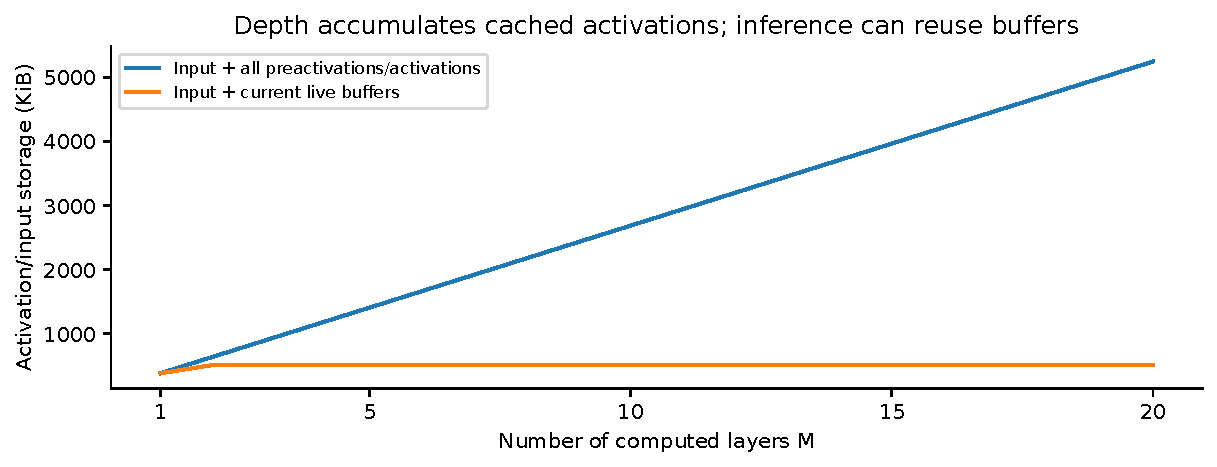
\includegraphics[width=\linewidth]{mlp_1_4_1_5/activation_memory.pdf}
\caption{Storage for input and activations at $B=512$, $d=k=64$. The cached implementation stores both $Z$ and $H$ for every layer. The inference model retains the input and only live layer buffers. Parameters are excluded from this plot to isolate activation lifetime; they must be added for total memory. These are calculated array sizes, not measured runtime allocations.}
\end{figure}

Do not sum each layer's full memory formula mechanically and count the same weights or boundary activation twice as distinct objects. Count distinct stored arrays, then decide which coexist. Likewise, multiplying a $B\times d$ batch by a $d\times k$ matrix does not require a $B\times d\times k$ tensor of all scalar products; standard matrix multiplication accumulates into the $B\times k$ output.

\paragraph{What happens to the expanded bias?}
Mathematically $\mathbf1_B\mathbf{b}^{\mathsf T}$ has $Bk$ entries, but broadcasting need not allocate a separate dense repeated copy. There remain only $k$ learned bias parameters. Explicitly materializing the repeated matrix adds a $Bk$ temporary; the activation order is unchanged, but practical memory use increases.

\begin{figure}[htbp]
\centering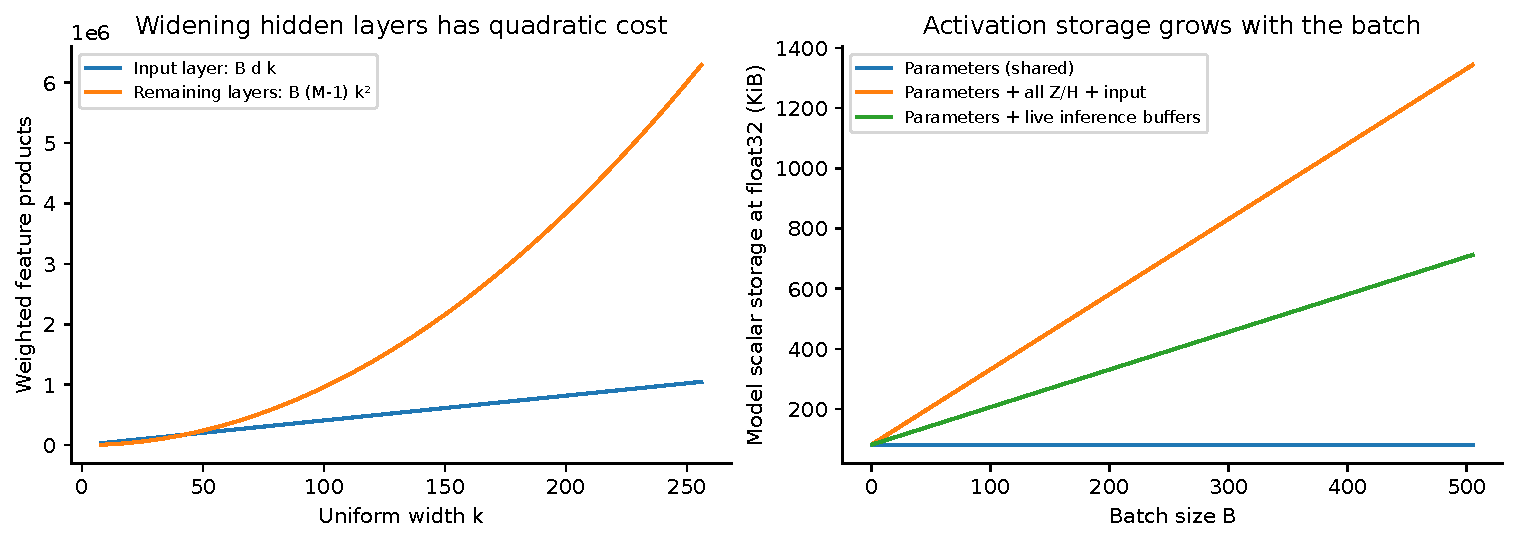
\includegraphics[width=\linewidth]{mlp_1_4_1_5/complexity_scaling.pdf}
\caption{Left: ordinary multiplication counts for four width-$k$ computed layers, $B=32$, $d=128$. Right: a four-layer model with $d=128$, $k=64$ and variable batch size. Weights are reused across examples, while activation/input storage grows with $B$. Curves are analytic counts, not timing measurements.}
\end{figure}

\subsection{A numerical batch budget and what it teaches}
Return to the $12\to32\to16\to1$ grasp model. At $B=256$, the input has 3,072 entries and all $Z/H$ arrays have $2(256)(49)=25,088$ entries. Including 961 parameters yields
\[
 S_{\mathrm{cache}}=29{,}121\text{ scalars}=116{,}484\text{ bytes at float32}.
\]
One conservative inference implementation, keeping the input plus separate live input/$Z$/$H$ buffers, peaks at 16,384 live intermediate scalars, hence
\[
 S_{\mathrm{infer}}=961+3{,}072+16{,}384=20{,}417\text{ scalars}.
\]
The live intermediate maximum is attained by $2B(32)$ in the first layer or $B(32+2\cdot16)$ in the second. In-place activation or fused kernels can reduce this number. These precise counts belong to the stated storage model, whereas the big-O expressions describe scaling robustly across such constant-factor changes.

Larger batches increase arithmetic and activation storage but not parameter count. Wider hidden layers can increase matrix work quadratically because both ends of a dense connection grow. More layers increase weight storage and computation approximately linearly at fixed width; retained activations also accumulate with depth. These observations help reason about embedded inference and GPU batch sizing before running an experiment.

\subsection{NumPy implementation: translate the equations literally}
\begin{lstlisting}
import numpy as np

X = np.array([[1., 2., 3.], [-1., 0., 2.]])  # (B=2, d=3)
W = np.array([[1., -1., 2.], [0., 3., -1.]]) # (q=2, d=3)
b = np.array([0.5, -0.5])                    # (q=2,)
Z = X @ W.T + b                             # (B=2, q=2)
H = np.maximum(Z, 0.0)                      # (B=2, q=2)
np.testing.assert_allclose(Z, [[5.5, 2.5], [3.5, -2.5]])

# The same calculation in the slide convention:
Xc = X.T                                   # (d=3, B=2)
Ws = W.T                                   # (d=3, q=2)
Zc = Ws.T @ Xc + b[:, None]                 # (q=2, B=2)
np.testing.assert_allclose(Z, Zc.T)
\end{lstlisting}
For a network, each layer consumes the previous layer's output:
\begin{lstlisting}
H = X
for ell, (W, b) in enumerate(zip(weights, biases)):
    Z = H @ W.T + b
    if ell < len(weights) - 1:
        H = np.maximum(Z, 0.0)              # hidden ReLU
    else:
        H = np.exp(-np.logaddexp(0.0, -Z)) # stable sigmoid
\end{lstlisting}
This code assumes a binary or independent-sigmoid output, not a mutually exclusive multiclass softmax. No labels are needed to produce predictions. Labels enter when computing a loss.

Beware of \texttt{X * W}: it is elementwise multiplication, not a collection of dot products. Also, \texttt{np.zeros(d).T} still has shape \texttt{(d,)}; transpose does not turn a one-dimensional array into a column. Use \texttt{x[:, None]} for \texttt{(d,1)} or \texttt{x[None, :]} for \texttt{(1,d)}. For loss calculations, keep both targets and predictions consistently \texttt{(B,)} or consistently \texttt{(B,1)}: subtracting arrays of these two different shapes can silently create a \texttt{(B,B)} result.

\subsection{Exercises with worked answers}
\paragraph{1. Recover the matrix dimensions.}
A batch has 8 examples with 6 features and a layer has 5 neurons. In row notation,
$X:8\times6$, $W:5\times6$, $b:5$, $Z,H:8\times5$.
In column notation, $X_c:6\times8$, $W_s:6\times5$, and $Z_c,H_c:5\times8$.
Both compute 240 scalar weight products and use 35 trainable parameters.

\paragraph{2. Check the boundary cases of the complexity answer.}
At $M=1$, $T=O(Bdk)$, and inclusive memory is $O(dk+k+Bd+Bk)$. At $B=1$, the general batch formulas reduce to single-example formulas. If $d=k$ and $M\geq1$, time simplifies to $O(BMk^2)$. Checking these cases can reveal an incorrectly counted input layer or an extra hidden layer.

\paragraph{3. Does doubling batch size double total memory?}
Write $S=P+A(B)$ where $P$ is fixed parameter storage and $A(B)$ is linear in $B$ under a fixed buffering policy. Then $S(2B)=P+2A(B)$, which is generally less than $2S(B)$. It approaches twice as much only when batch-dependent storage dominates.

\paragraph{4. Why not multiply the parameter count by B?}
A parameter defines the same function for every example. Batching evaluates that one function repeatedly. For an ordinary MLP, permuting the batch rows permutes output rows in exactly the same way; it does not change the parameters or mix information between examples.

\paragraph{5. Why can a shape-correct expression still be wrong?}
If $B=d=q$, several incorrect transposes and bias placements produce compatible square shapes. They can combine examples instead of features or associate biases with examples. Evaluate a small nonsquare example against scalar loops to test the intended index semantics. The companion script checks this equivalence, verifies row/column conversion, and compares batched predictions with one-example-at-a-time predictions.

\paragraph{Reproducible companion.}
Run \texttt{python deep\_learning/code/mlp\_1\_4\_1\_5.py} from the repository root. It verifies the numerical examples and parameter/cache counts, demonstrates affine collapse and XOR, and regenerates all four figures. Its memory plots count array elements under explicit buffering assumptions and do not claim measured CPU/GPU memory or latency.

% ============================================================
%  1.6 Other Activation Functions and Loss Functions
% ============================================================
\section{Other Activation Functions and Loss Functions}
\label{sec:logreg_to_mlp:other_activation_functions_and_loss_functions}

% Notes go here.

% ============================================================
%  1.7 Representational Power of MLPs
% ============================================================
\section{Representational Power of MLPs}
\label{sec:logreg_to_mlp:representational_power_of_mlps}

% Notes go here.

% ============================================================
%  1.8 Summary, Further Reading, References
% ============================================================
\section{Summary, Further Reading, References}
\label{sec:logreg_to_mlp:summary_further_reading_references}

% Notes go here.


% ============================================================
%  Chapter 2: MLPs and Backpropagation
% ============================================================
\chapter{MLPs and Backpropagation}
\label{ch:mlp_backprop}

% ============================================================
%  2.1 Recap of Multilayer Perceptrons
% ============================================================
\section{Recap of Multilayer Perceptrons}
\label{sec:mlp_backprop:recap_of_multilayer_perceptrons}

% Notes go here.

% ============================================================
%  2.2 Recap of Chain Rule of Calculus
% ============================================================
\section{Recap of Chain Rule of Calculus}
\label{sec:mlp_backprop:recap_of_chain_rule_of_calculus}

% Notes go here.

% ============================================================
%  2.3 Calculating Gradients with Backpropagation
% ============================================================
\section{Calculating Gradients with Backpropagation}
\label{sec:mlp_backprop:calculating_gradients_with_backpropagation}

% Notes go here.

% ============================================================
%  2.4 Backprop for a Linear Layer in Matrix Form
% ============================================================
\section{Backprop for a Linear Layer in Matrix Form}
\label{sec:mlp_backprop:backprop_for_a_linear_layer_in_matrix_form}

% Notes go here.

% ============================================================
%  2.5 Full Matrix Form of Backpropagation Equations
% ============================================================
\section{Full Matrix Form of Backpropagation Equations}
\label{sec:mlp_backprop:full_matrix_form_of_backpropagation_equations}

% Notes go here.

% ============================================================
%  2.6 Summary, Further Reading, References
% ============================================================
\section{Summary, Further Reading, References}
\label{sec:mlp_backprop:summary_further_reading_references}

% Notes go here.



% ---------------- Bibliography ----------------
\bibliographystyle{plainnat}
% Course textbooks; remove once you cite things with \cite{...}
\nocite{goodfellow2016deep}
\bibliography{references}

\end{document}
